\newpage
%%%%%%%%%%%%%%%%%%%%%%%%%%%%%%%%%%%%%%%%%%%%%
%%% Chapter 2: DORI - Hardware Development
%%%%%%%%%%%%%%%%%%%%%%%%%%%%%%%%%%%%%%%%%%%%%
\chapter{Hardware Development}
\label{chapter:hardware_development}
This chapter describes the development of the DORI (\textit{DOs\'imetro para Radiologia de Interven\c{c}\~ao}) prototype, designed in response to the previously identified limitations. The conceptual design of the system is shown in Fig.~\ref{fig:DORI}.
\begin{figure}[H]
  \centering
  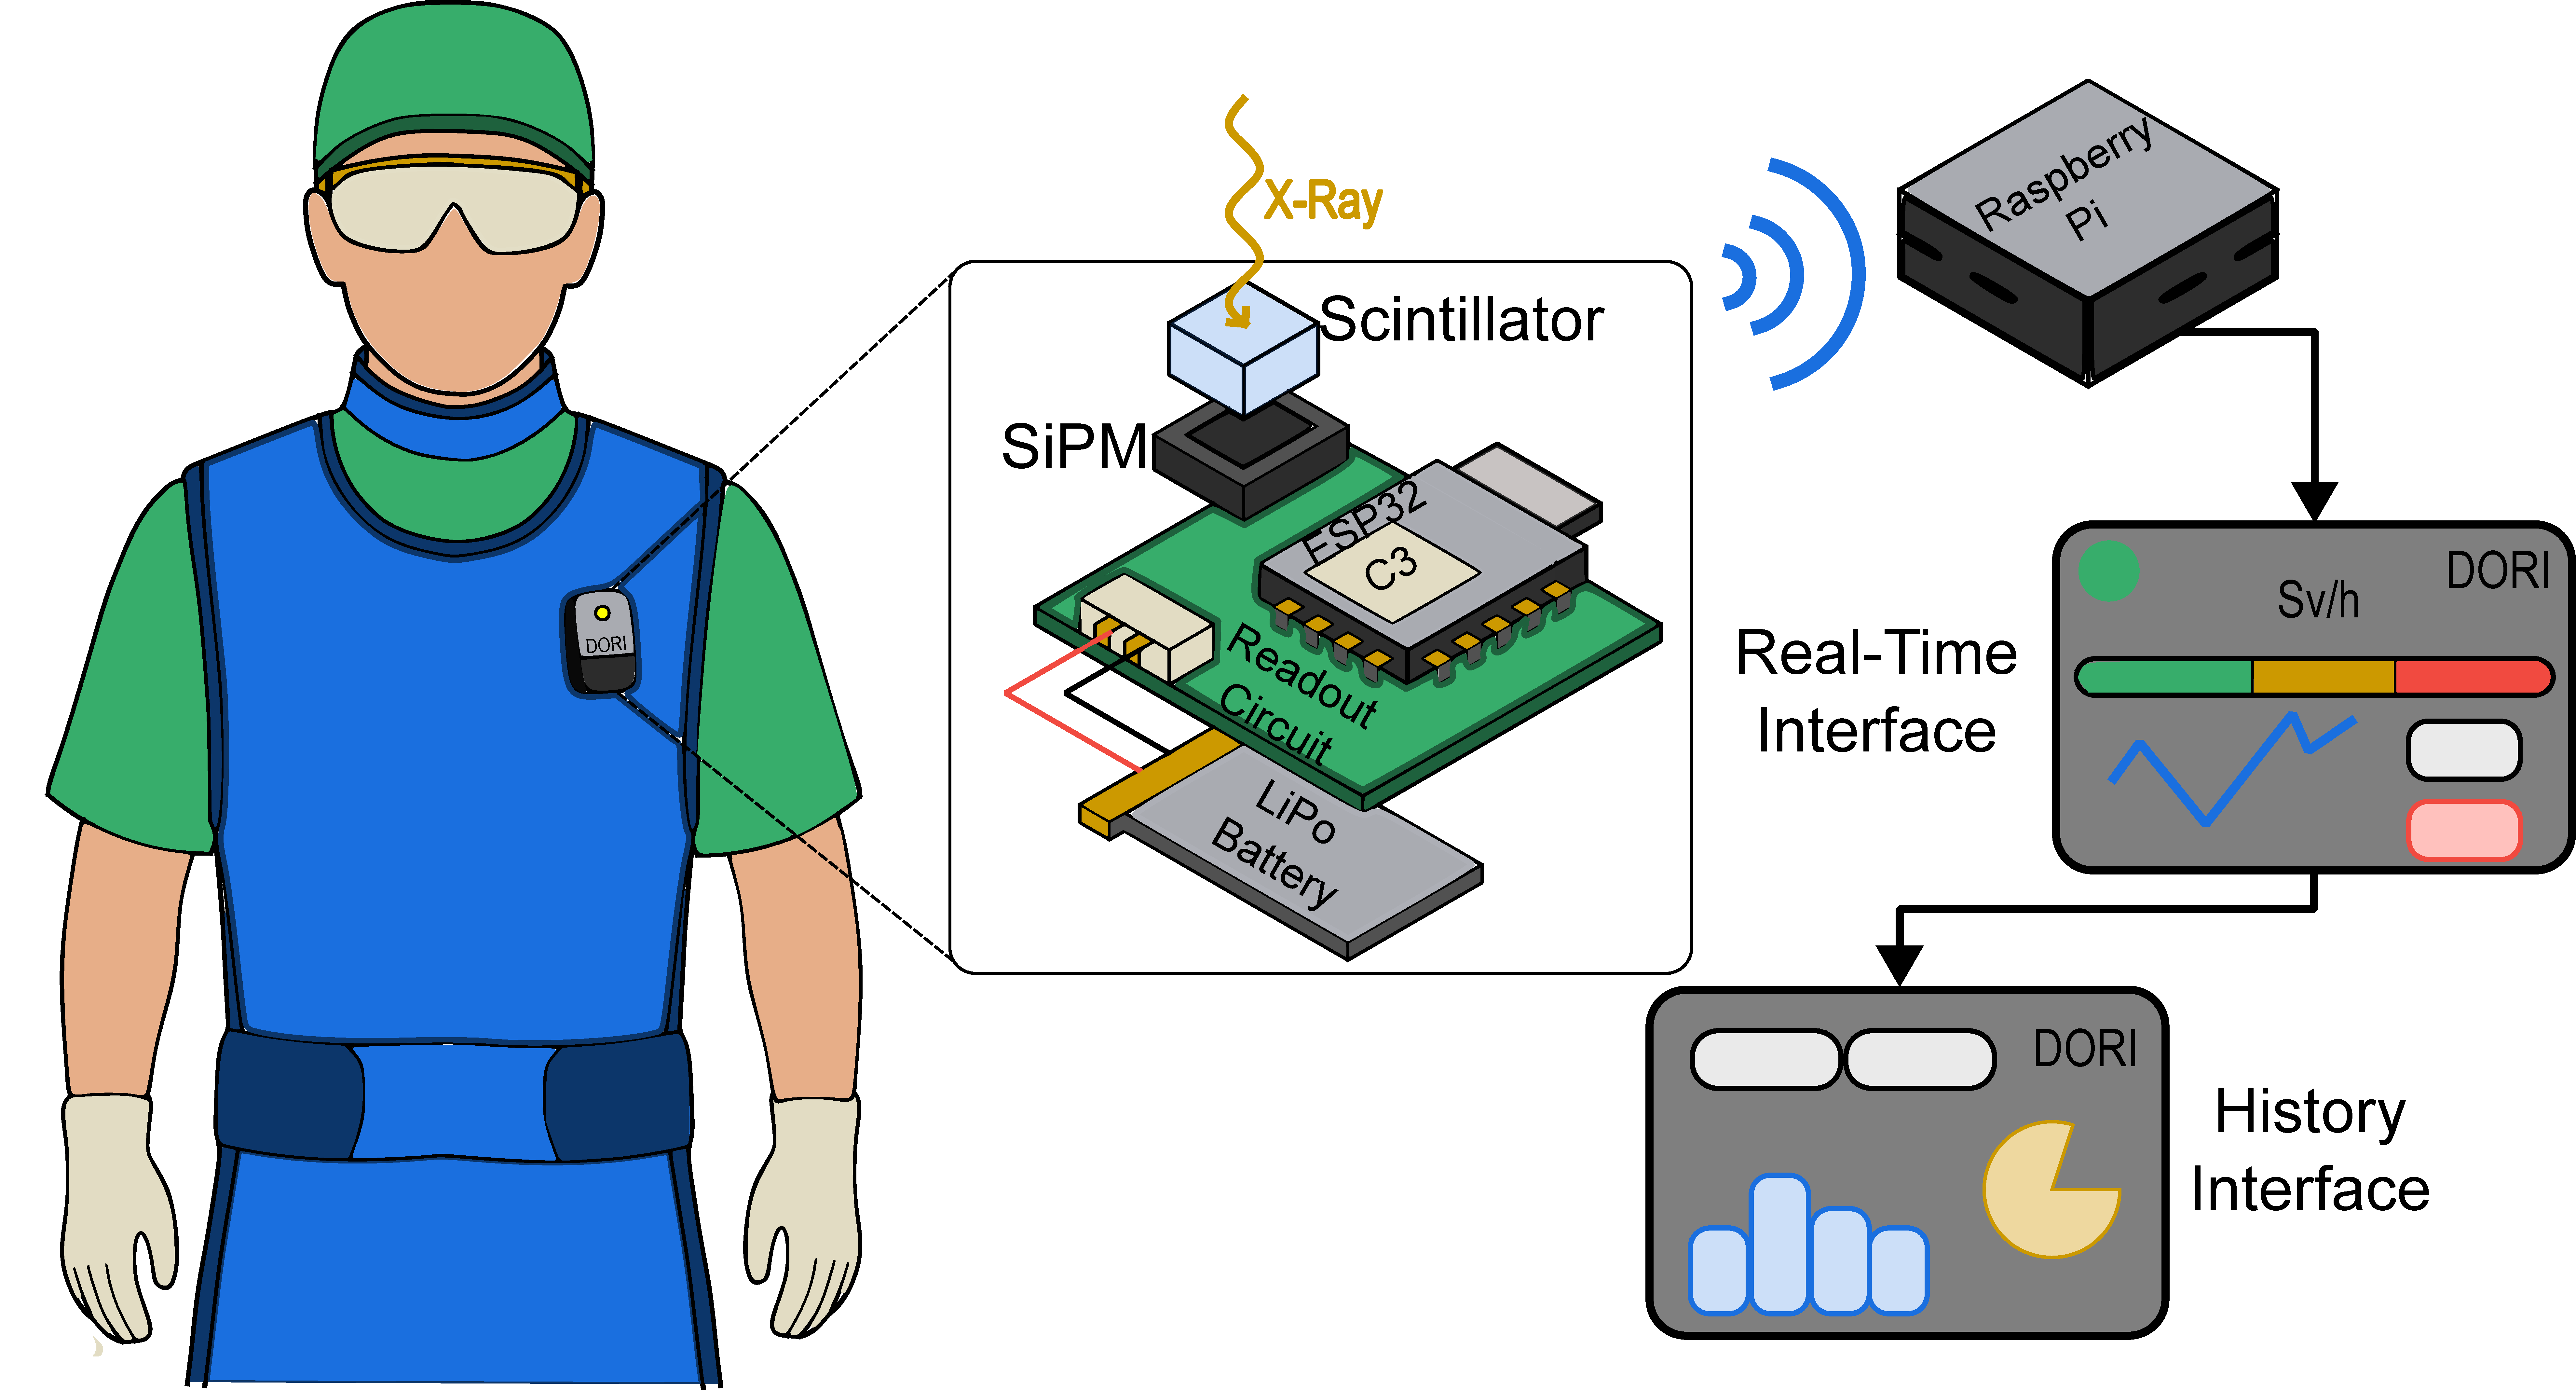
\includegraphics[width=\linewidth]{images/DORI.pdf}
  \caption[Conceptual design of DORI.]{Conceptual design of DORI. The wearable unit (exploded
view) is worn over the protective apron and comprises the scintillator,
photodetector, readout circuit, MCU and LiPo battery. Data are sent to a
Raspberry Pi, which displays the real-time and history interfaces.}
  \label{fig:DORI}
\end{figure}
DORI consists of a compact wearable unit, worn over the protective apron, which integrates the full detection, pulse processing and transmission chain. Each stage is described in detail in the following sections. In general terms, scattered radiation interacts with a scintillator, and the resulting light is converted into an electrical signal by a photodetector.
DORI operates in pulse mode, where each interaction is registered as an individual event. The corresponding pulse is conditioned by a readout board, which preserves the amplitude and thereby the energy deposited in each event. By accounting for the energy of individual interactions, rather than integrating total charge, the accuracy of the dose calculation can be improved. The target energy range is 20 to 100~keV, corresponding to the energies of the scattered field in IR (recall Table~\ref{tab:ir_parameters}).

The chain is controlled by a microcontroller unit (MCU) with wireless communication capabilities. The ESP32-C3 was selected for being compact, lightweight and low-cost. It supports 2.4~GHz Wi-Fi and Bluetooth\textsuperscript{\textregistered} Low Energy (BLE)~5~\cite{134}, the latter being the adopted communication protocol. Unlike Wi-Fi, BLE establishes a direct link with the receiver and requires no external router, reducing system complexity. In addition, BLE~5 offers extended range and increased data throughput relative to previous versions, meeting the requirements of continuous dose transmission. The unit is powered by a rechargeable lithium polymer (LiPo) battery, the AKYGA LP103040~\cite{135}, whose 1200~mAh capacity supports uninterrupted operation over extended periods. The selected Seeed Studio XIAO ESP32-C3~\cite{133} board already incorporates a charging circuit for the battery via its USB-C port. Accordingly, the front-end electronics operate at a 3.3~V logic level.

To preserve battery life, the wearable unit does not compute dose. The MCU accumulates the amplitude information of the detected events and transmits it via BLE at a one-second rate to a Raspberry Pi. Since the Raspberry Pi is permanently powered, it handles all data processing, from pulse amplitude to energy and, ultimately, to dose. A real-time interface then displays the dose rate with a complementary colour-coded scale, updated at the same one-second rate. The scale is replicated on an LED integrated in the wearable unit, with the corresponding colour level sent back to the badge via BLE. All measured data are also stored in an internal database, from which a second interface builds retrospective summaries of the recorded exposure.
\section{Scintillator}
\label{sec:scintillator}
The detection of the scattered radiation is based on a plastic scintillator (PS). PSs are organic materials that emit photons in the near ultraviolet to visible range when excited by ionising radiation. The selected scintillator is a $5 \times 5 \times 5$~mm$^3$ BC-408 cube. BC-408 consists of a polyvinyltoluene base doped with fluorophore compounds that shift the emission to a peak wavelength of 425~nm~\cite{128}.

The main advantage of PSs is their tissue equivalence. Their effective atomic number is also lower than that of the materials used in passive dosimeters or in solid-state diodes, like the RaySafe i3. The energy absorbed in the scintillator therefore approximates the dose to soft tissue without requiring further corrections~\cite{129}. However, as a drawback, the same tissue equivalence implies that, as in soft tissue, Compton scattering predominates over the photoelectric effect at the photon energies of the scattered field. From an energy calibration perspective, the acquired spectrum reduces to a Compton continuum without photopeaks, and the standard identification of $\gamma$-emitting radionuclides is not possible (recall Section~\ref{sec:Photon Interaction with Matter}). Consequently, the energy resolution of these detectors is poor. The only identifiable spectral feature is the CE, corresponding to the maximum energy transfer at a scattering angle of $\theta = 180^{\circ}$, whose energy is well known for a given source through Eq.\ref{eq:compton}. Nonetheless, owing to the poor energy resolution at the energies of interest, the CE may not coincide with the channel of maximum counts. To resolve this ambiguity, Compton coincidence techniques are employed, in which the backscattered photon from a CE event is detected in coincidence with a reference detector. However, these have primarily been demonstrated using $^{22}$Na and $^{137}$Cs, whose CEs lie outside the range relevant to this work~\cite{127}.

Such methods also assume a proportional response, meaning a light output that scales linearly with the deposited energy. However, below approximately 125~keV, the light output of PSs is non-proportional due to ionisation quenching. Slow (lower energy) electrons ionise the medium more densely, and part of the excitation is dissipated without the emission of light~\cite{130}. The Compton electrons produced in the PS in this work fall below this threshold. The pulse height of the detected events may therefore not be a linear measure of the deposited energy, and the response must instead be characterised locally, with any calibration valid only within the region where it is established.
\section{Photodetector}
To detect the scintillation light and convert it into an electrical signal, a silicon photomultiplier (SiPM) from Broadcom (AFBR-S4N66P014M~\cite{131}) was optically coupled to the scintillator. Its $6\times6$~mm\textsuperscript{2} active area matches the PS cross section, maximizing light collection. Additionally, the photon detection efficiency of the SiPM peaks at 420~nm, close to the peak emission of BC-408~\cite{131}.

A SiPM consists of a parallel array of avalanche photodiodes operated in Geiger mode. Each cell is reverse biased above its breakdown voltage, so a single absorbed photon is sufficient to trigger a self-sustaining avalanche. The photons produced by a scintillation event fire many pixels simultaneously, each of which contributes one identical pulse. The summed output current is proportional to the number of fired cells, and therefore to the energy deposited in the PS~\cite{14}. The number of available microcells (22\,428) fulfills the requirements given the photons produced per scintillation event. The SiPM has a breakdown voltage of 33~V and supports overvoltages of up to 16~V~\cite{131}.

\subsection{SiPM Power Supply}
\label{sec:sipm_power_supply}
The SiPM operating voltage was set to 37~V. Although gain increases with overvoltage, so do the dark count rate and crosstalk probability, which in excess mask the low-energy end of the spectrum. For the 20 to 100~keV range, an overvoltage of 4~V provides enough gain for these events to sit above noise levels. The bias is generated by a MAX1932 ~\cite{132} and its output is programmed through a Serial Peripheral Interface (SPI) by the MCU, which writes an eight-bit code to the internal DAC of the power supply.

A fixed 37~V output does not account for the variation of the breakdown voltage with temperature, which increases at 30~mV/$^\circ$C according to the SiPM datasheet~\cite{131}. Since gain depends on the overvoltage, a constant bias means the gain decreases as temperature rises. The same deposited energy then produces a different pulse amplitude, affecting the energy calibration and the derived dose. To compensate for this, an NTC thermistor was added to the feedback network, as recommended in the MAX1932 datasheet~\cite{132} and shown in Fig.~\ref{fig:bias}. The total resistance between the FB node and ground is~\cite{132}:
\begin{equation}
R_\text{total}(T) = R_8 + \frac{R_9\,R_T(T)}{R_9 + R_T(T)},
\label{eq:rtotal}
\end{equation}
The output voltage is therefore~\cite{132}:
\begin{equation}
V_\text{OUT} = 1.25\left(1 + \frac{R_5}{R_\text{total}(T)}\right) + \frac{R_5}{R_6}\left(1.25 - V_\text{DAC}\right),
\label{eq:vout_max}
\end{equation}
where $V_\text{DAC}$ is the DAC output voltage. The compensation condition requires the derivative of Eq.~\ref{eq:vout_max} to equal the temperature coefficient of the breakdown voltage over the operating range of 18 to 25~$^\circ$C:
\begin{equation}
\frac{dV_\text{OUT}}{dT} = \frac{1.25\,R_5}{R_\text{total}^2}\left(\frac{R_9}{R_9 + R_T}\right)^2 \frac{\beta}{T^2}\,R_T = 30~\text{mV/}^\circ\text{C}.
\label{eq:slope}
\end{equation}
Solving this condition together with Eqs.~\ref{eq:rtotal} and \ref{eq:vout_max} and the component selection equations of the datasheet~\cite{132} yields $R_5 = 91$~k$\Omega$, $R_6 = 27$~k$\Omega$, $R_8 = 2.4$~k$\Omega$, and $R_9 = 910$~$\Omega$.
\begin{figure}[H]
  \centering
  \resizebox{!}{5.2cm}{\tikzset{every picture/.style={line width=0.75pt}} %set default line width to 0.75pt        

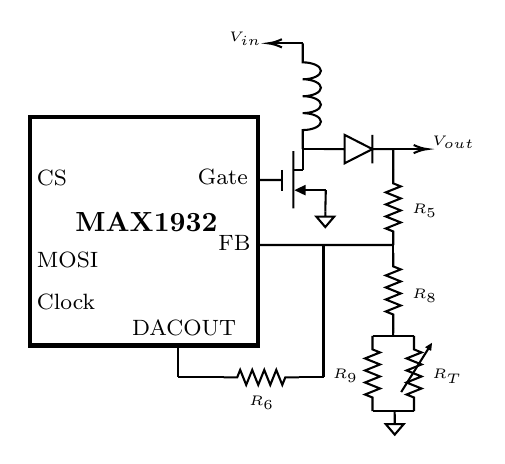
\begin{tikzpicture}[x=0.75pt,y=0.75pt,yscale=-1,xscale=1]
%uncomment if require: \path (0,300); %set diagram left start at 0, and has height of 300

%Shape: Square [id:dp45442051822513774] 
\draw  [line width=1.5]  (218.47,64.6) -- (328.47,64.6) -- (328.47,174.6) -- (218.47,174.6) -- cycle ;
%Shape: Inductor (Air Core) [id:dp8320962493713222] 
\draw   (350,29.04) -- (350,38.21) .. controls (354.83,38.21) and (358.75,40.04) .. (358.75,42.29) .. controls (358.75,44.54) and (354.83,46.37) .. (350,46.37) .. controls (354.83,46.37) and (358.75,48.19) .. (358.75,50.44) .. controls (358.75,52.69) and (354.83,54.52) .. (350,54.52) .. controls (354.83,54.52) and (358.75,56.35) .. (358.75,58.6) .. controls (358.75,60.85) and (354.83,62.67) .. (350,62.67) .. controls (354.83,62.67) and (358.75,64.5) .. (358.75,66.75) .. controls (358.75,69) and (354.83,70.83) .. (350,70.83) -- (350,80) ;
%Shape: Diode [id:dp522086168972487] 
\draw   (370.19,73.17) -- (383.57,80) -- (370.19,86.83) -- (370.19,73.17) -- cycle (360.16,80) -- (370.19,80) (383.57,73.17) -- (383.57,86.83) (383.57,80) -- (393.6,80) ;
%Shape: Resistor [id:dp8144600229276032] 
\draw   (393.61,90) -- (393.61,96.52) -- (397.22,97.97) -- (390,100.86) -- (397.22,103.76) -- (390,106.66) -- (397.22,109.55) -- (390,112.45) -- (397.22,115.35) -- (390,118.24) -- (393.61,119.69) -- (393.61,126.21) ;
%Straight Lines [id:da29049231672487486] 
\draw    (340,90) -- (340,100) ;
%Straight Lines [id:da4316288408593886] 
\draw    (361.11,99.78) -- (348.99,99.78) ;
\draw [shift={(345.99,99.78)}, rotate = 360] [fill={rgb, 255:red, 0; green, 0; blue, 0 }  ][line width=0.08]  [draw opacity=0] (5.36,-2.57) -- (0,0) -- (5.36,2.57) -- cycle    ;
%Straight Lines [id:da6953106373785519] 
\draw    (361.11,99.78) -- (360.86,110) ;
%Shape: Ground [id:dp011205472514209114] 
\draw   (356.54,112.52) -- (360.86,117.56) -- (365.17,112.52) -- (356.54,112.52) -- cycle (360.86,110) -- (360.86,112.52) ;
%Straight Lines [id:da5829290803316644] 
\draw    (350,80) -- (360.16,80) ;
%Straight Lines [id:da05768888846435982] 
\draw    (345.48,80.94) -- (345.5,108.61) ;
%Straight Lines [id:da31478243553340524] 
\draw    (350,80) -- (350,90) ;
%Straight Lines [id:da2330593515607322] 
\draw    (350,90) -- (345.79,90) ;
%Straight Lines [id:da3584287863409543] 
\draw    (328.59,94.89) -- (340.16,94.88) ;
%Shape: Resistor [id:dp4537216327878536] 
\draw   (393.61,130) -- (393.61,136.52) -- (397.22,137.97) -- (390,140.86) -- (397.22,143.76) -- (390,146.66) -- (397.22,149.55) -- (390,152.45) -- (397.22,155.35) -- (390,158.24) -- (393.61,159.69) -- (393.61,166.21) ;
%Shape: Resistor [id:dp44213159457902096] 
\draw   (383.61,170) -- (383.61,176.52) -- (387.22,177.97) -- (380,180.86) -- (387.22,183.76) -- (380,186.66) -- (387.22,189.55) -- (380,192.45) -- (387.22,195.35) -- (380,198.24) -- (383.61,199.69) -- (383.61,206.21) ;
%Shape: Resistor [id:dp5279058570816227] 
\draw   (403.61,170) -- (403.61,176.52) -- (407.22,177.97) -- (400,180.86) -- (407.22,183.76) -- (400,186.66) -- (407.22,189.55) -- (400,192.45) -- (407.22,195.35) -- (400,198.24) -- (403.61,199.69) -- (403.61,206.21) ;
%Shape: Ground [id:dp21864911769776485] 
\draw   (390,212.52) -- (394.31,217.56) -- (398.63,212.52) -- (390,212.52) -- cycle (394.31,210) -- (394.31,212.52) ;
%Shape: Resistor [id:dp5330487161197813] 
\draw   (311.9,190) -- (318.41,190) -- (319.86,186.39) -- (322.76,193.61) -- (325.65,186.39) -- (328.55,193.61) -- (331.45,186.39) -- (334.35,193.61) -- (337.24,186.39) -- (340.14,193.61) -- (341.59,190) -- (348.1,190) ;
%Straight Lines [id:da903277102568916] 
\draw    (397.43,197.05) -- (410.69,175.88) ;
\draw [shift={(412.29,173.33)}, rotate = 122.07] [fill={rgb, 255:red, 0; green, 0; blue, 0 }  ][line width=0.08]  [draw opacity=0] (3.57,-1.72) -- (0,0) -- (3.57,1.72) -- cycle    ;
%Straight Lines [id:da6627028399578476] 
\draw    (393.61,126.21) -- (393.61,130) ;
%Straight Lines [id:da19956176075595244] 
\draw    (383.61,170) -- (403.61,170) ;
%Straight Lines [id:da9867546245054489] 
\draw    (393.61,166.21) -- (393.56,170.39) ;
%Straight Lines [id:da699703638594996] 
\draw    (383.61,206.21) -- (403.61,206.21) ;
%Straight Lines [id:da6230017749012404] 
\draw    (394.3,206.05) -- (394.31,210) ;
%Straight Lines [id:da5942027422502576] 
\draw    (393.61,90) -- (393.6,80) ;
%Straight Lines [id:da7853613457386626] 
\draw    (393.61,126.21) -- (328.37,126.2) ;
%Straight Lines [id:da6727874772719629] 
\draw    (290,174.57) -- (290,190) ;
%Straight Lines [id:da9301720203284228] 
\draw    (311.9,190) -- (290,190) ;
%Straight Lines [id:da23173374113205025] 
\draw    (360,126.43) -- (360,190) ;
%Straight Lines [id:da39088728409946005] 
\draw    (348.1,190) -- (360,190) ;
%Straight Lines [id:da34090922258728096] 
\draw    (350,29.04) -- (335.39,29.04) ;
\draw [shift={(333.39,29.04)}, rotate = 360] [color={rgb, 255:red, 0; green, 0; blue, 0 }  ][line width=0.75]    (6.56,-1.97) .. controls (4.17,-0.84) and (1.99,-0.18) .. (0,0) .. controls (1.99,0.18) and (4.17,0.84) .. (6.56,1.97)   ;
%Straight Lines [id:da06307080945568311] 
\draw    (390,80) -- (408,80) ;
\draw [shift={(410,80)}, rotate = 180] [color={rgb, 255:red, 0; green, 0; blue, 0 }  ][line width=0.75]    (6.56,-1.97) .. controls (4.17,-0.84) and (1.99,-0.18) .. (0,0) .. controls (1.99,0.18) and (4.17,0.84) .. (6.56,1.97)   ;

% Text Node
\draw (298,88.22) node [anchor=north west][inner sep=0.75pt]  [font=\small] [align=left] {{\footnotesize Gate}};
% Text Node
\draw (307.9,120.17) node [anchor=north west][inner sep=0.75pt]  [font=\small] [align=left] {{\footnotesize FB}};
% Text Node
\draw (266.24,160.79) node [anchor=north west][inner sep=0.75pt]  [font=\small] [align=left] {{\footnotesize DACOUT}};
% Text Node
\draw (220.44,88.89) node [anchor=north west][inner sep=0.75pt]  [font=\small] [align=left] {{\footnotesize CS}};
% Text Node
\draw (220.44,128.33) node [anchor=north west][inner sep=0.75pt]  [font=\small] [align=left] {{\footnotesize MOSI}};
% Text Node
\draw (220.44,148.56) node [anchor=north west][inner sep=0.75pt]  [font=\small] [align=left] {{\footnotesize Clock}};
% Text Node
\draw (239,109) node [anchor=north west][inner sep=0.75pt]   [align=left] {\textbf{MAX1932}};
% Text Node
\draw (313,22) node [anchor=north west][inner sep=0.75pt]  [font=\tiny] [align=left] {$V_{\text{in}}$};
% Text Node
\draw (411,72) node [anchor=north west][inner sep=0.75pt]  [font=\tiny] [align=left] {$V_{\text{out}}$};
% Text Node
\draw (401.22,105.01) node [anchor=north west][inner sep=0.75pt]  [font=\tiny] [align=left] {$R_5$};
% Text Node
\draw (401.22,145.9) node [anchor=north west][inner sep=0.75pt]  [font=\tiny] [align=left] {$R_8$};
% Text Node
\draw (411,184.49) node [anchor=north west][inner sep=0.75pt]  [font=\tiny] [align=left] {$R_{\text{T}}$};
% Text Node
\draw (363,184.49) node [anchor=north west][inner sep=0.75pt]  [font=\tiny] [align=left] {$R_9$};
% Text Node
\draw (322.67,197.6) node [anchor=north west][inner sep=0.75pt]  [font=\tiny] [align=left] {$R_6$};

\end{tikzpicture}}
  \caption[SiPM bias supply.]{MAX1932 feedback network with the NTC thermistor $R_T$ for temperature compensation of the SiPM bias. Pin labels on the left correspond to SPI connections.}
  \label{fig:bias}
\end{figure}



\section{Front-End Electronics}
\label{sec:front_end}
The front-end electronics perform the pulse-mode readout of the SiPM response. The architecture developed for this purpose is represented by the simplified block diagram in Fig.~\ref{fig:architecture}, and includes three stages. Pulse shaping integrates and filters the SiPM current into a voltage pulse whose amplitude is proportional to the collected charge. Pulse discrimination then compares this pulse against a reference threshold, rejecting noise, and retains its peak amplitude. Pulse sampling digitises the held value through an Analog-to-Digital Converter (ADC) and transmits it to the MCU. Each stage is detailed in the following sections.

The front-end electronics were assembled on a printed circuit board (PCB), which also integrates the ESP32-C3, the MAX1932 bias supply and the SiPM described previously. The DORI-test board is shown in Fig.~\ref{fig:pcb} (a). The scintillator and the SiPM are not soldered directly on the board. Instead, the two are optically coupled and enclosed in an individual light-tight printed box, connected to the readout chain through a pin header. This arrangement allows the detector elements to be replaced without reworking the board, so that different configurations can be evaluated with the same electronics. All measurements presented in this work were performed with three sealed radioactive sources, $^{241}$Am, $^{109}$Cd and $^{57}$Co, selected because their emissions fall within the energy range of interest. Further information on their activities can be found in Appendix~A. A test box was 3D printed to align each source with the active area of the photosensitive housing, as shown in Fig.~\ref{fig:pcb} (b). The box additionally reduces the handling of the sources and allows a greater distance to be maintained during testing, contributing to a lower radiation exposure.
\begin{figure}[H]
  \centering
  \resizebox{\linewidth}{!}{

\tikzset{every picture/.style={line width=0.75pt}} %set default line width to 0.75pt        

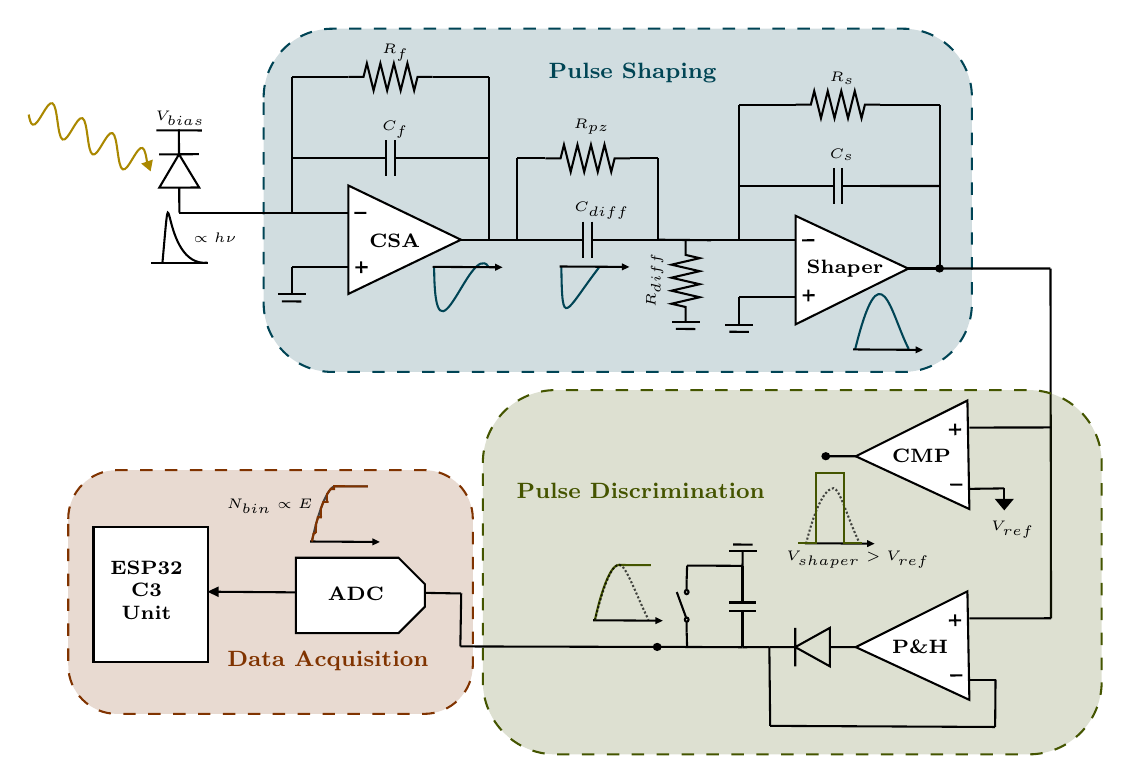
\begin{tikzpicture}[x=0.75pt,y=0.75pt,yscale=-1,xscale=1]
%uncomment if require: \path (0,390); %set diagram left start at 0, and has height of 390

%Rounded Rect [id:dp46800229916678826] 
\draw  [color={rgb, 255:red, 128; green, 51; blue, 0 }  ,draw opacity=1 ][fill={rgb, 255:red, 128; green, 51; blue, 0 }  ,fill opacity=0.18 ][dash pattern={on 4.5pt off 4.5pt}] (75.7,255.44) .. controls (75.7,242.46) and (86.22,231.95) .. (99.19,231.95) -- (247.14,231.95) .. controls (260.12,231.95) and (270.63,242.46) .. (270.63,255.44) -- (270.63,325.9) .. controls (270.63,338.88) and (260.12,349.39) .. (247.14,349.39) -- (99.19,349.39) .. controls (86.22,349.39) and (75.7,338.88) .. (75.7,325.9) -- cycle ;
%Rounded Rect [id:dp6060718292152891] 
\draw  [color={rgb, 255:red, 0; green, 68; blue, 85 }  ,draw opacity=1 ][fill={rgb, 255:red, 0; green, 68; blue, 85 }  ,fill opacity=0.18 ][dash pattern={on 4.5pt off 4.5pt}] (169.85,52.35) .. controls (169.85,34.09) and (184.66,19.28) .. (202.92,19.28) -- (478.01,19.28) .. controls (496.28,19.28) and (511.09,34.09) .. (511.09,52.35) -- (511.09,151.57) .. controls (511.09,169.84) and (496.28,184.64) .. (478.01,184.64) -- (202.92,184.64) .. controls (184.66,184.64) and (169.85,169.84) .. (169.85,151.57) -- cycle ;
%Straight Lines [id:da20418652663852965] 
\draw    (118.17,68.23) -- (140.04,68.31) ;
%Shape: Diode [id:dp9073484797643522] 
\draw   (119.56,95.88) -- (129.08,79.78) -- (138.77,95.78) -- (119.56,95.88) -- cycle (129.23,107.87) -- (129.17,95.83) (119.47,79.83) -- (138.68,79.73) (129.08,79.78) -- (129.01,67.74) ;
%Straight Lines [id:da29328469712985317] 
\draw    (129.23,107.87) -- (210.63,107.87) ;
%Shape: Triangle [id:dp7568885508488827] 
\draw  [fill={rgb, 255:red, 255; green, 255; blue, 255 }  ,fill opacity=1 ] (264.89,120.94) -- (210.63,147.08) -- (210.63,94.8) -- cycle ;
%Straight Lines [id:da4819348879555857] 
\draw    (210.63,134.01) -- (183.5,134.01) ;
%Straight Lines [id:da645749601403131] 
\draw    (183.5,147.08) -- (183.5,134.01) ;
%Straight Lines [id:da6803870332982462] 
\draw    (176.71,147.27) -- (190.28,147.27) ;
%Straight Lines [id:da005605298303441364] 
\draw    (178.65,150.63) -- (188.04,150.71) ;
%Straight Lines [id:da05308331089564988] 
\draw    (183.5,107.87) -- (183.5,81.73) ;
%Straight Lines [id:da020906030143946763] 
\draw    (183.5,42.51) -- (183.5,94.8) ;
%Shape: Resistor [id:dp7434947714198523] 
\draw   (210.63,42.51) -- (217.95,42.51) -- (219.58,35.98) -- (222.83,49.05) -- (226.09,35.98) -- (229.35,49.05) -- (232.6,35.98) -- (235.86,49.05) -- (239.11,35.98) -- (242.37,49.05) -- (244,42.51) -- (251.32,42.51) ;
%Shape: Capacitor [id:dp42145798620234975] 
\draw   (210.63,81.73) -- (228.94,81.73) (233.01,72.99) -- (233.01,90.46) (228.94,72.99) -- (228.94,90.46) (233.01,81.73) -- (251.32,81.73) ;
%Straight Lines [id:da34880193469214116] 
\draw    (210.63,42.51) -- (183.5,42.51) ;
%Straight Lines [id:da026503265572629386] 
\draw    (264.89,120.94) -- (292.02,120.94) ;
%Straight Lines [id:da9274117024294998] 
\draw    (278.45,42.51) -- (278.45,120.94) ;
%Straight Lines [id:da7747280381922488] 
\draw    (251.32,42.51) -- (278.45,42.51) ;
%Straight Lines [id:da1032408852686264] 
\draw    (183.5,81.73) -- (210.63,81.73) ;
%Straight Lines [id:da1423279487465121] 
\draw    (251.32,81.73) -- (278.45,81.73) ;
%Curve Lines [id:da7997259707368105] 
\draw [color={rgb, 255:red, 0; green, 0; blue, 0 }  ,draw opacity=1 ][fill={rgb, 255:red, 255; green, 255; blue, 255 }  ,fill opacity=1 ]   (121.09,132.03) .. controls (126.11,76.56) and (119.49,134.29) .. (142.8,132.03) ;
%Straight Lines [id:da9485003249156622] 
\draw    (115.67,132.03) -- (142.8,132.03) ;
%Curve Lines [id:da49583939836969093] 
\draw [color={rgb, 255:red, 0; green, 68; blue, 85 }  ,draw opacity=1 ]   (313.29,133.84) .. controls (313.63,164.72) and (314.85,155.96) .. (331.36,134.4) ;
%Shape: Resistor [id:dp18008683636522793] 
\draw   (305.58,81.73) -- (312.91,81.73) -- (314.54,75.19) -- (317.79,88.26) -- (321.05,75.19) -- (324.3,88.26) -- (327.56,75.19) -- (330.81,88.26) -- (334.07,75.19) -- (337.33,88.26) -- (338.95,81.73) -- (346.28,81.73) ;
%Straight Lines [id:da6245327821504196] 
\draw    (292.02,120.94) -- (292.02,81.73) ;
%Straight Lines [id:da9330542602485921] 
\draw    (292.02,81.73) -- (305.58,81.73) ;
%Straight Lines [id:da7057152830278173] 
\draw    (292.02,120.94) -- (305.58,120.94) ;
%Shape: Capacitor [id:dp8095550086511366] 
\draw   (305.58,120.94) -- (323.9,120.94) (327.97,112.21) -- (327.97,129.67) (323.9,112.21) -- (323.9,129.67) (327.97,120.94) -- (346.28,120.94) ;
%Straight Lines [id:da5386226934871385] 
\draw    (346.28,81.73) -- (359.84,81.73) ;
%Straight Lines [id:da7313083657794016] 
\draw    (346.28,120.94) -- (359.84,120.94) ;
%Straight Lines [id:da03131911441569635] 
\draw    (359.84,81.73) -- (359.84,120.94) ;
%Curve Lines [id:da7413273067238557] 
\draw [color={rgb, 255:red, 0; green, 68; blue, 85 }  ,draw opacity=1 ][line width=0.75]    (252,134.01) .. controls (252.17,187.85) and (269.17,121.74) .. (278,133.68) ;
%Shape: Triangle [id:dp6184826935280519] 
\draw  [fill={rgb, 255:red, 255; green, 255; blue, 255 }  ,fill opacity=1 ] (480.43,134.86) -- (426.17,161.72) -- (426.17,109.44) -- cycle ;
%Straight Lines [id:da31773246729249327] 
\draw    (426.17,148.65) -- (399.03,148.65) ;
%Straight Lines [id:da3550332613541024] 
\draw    (399.03,161.72) -- (399.03,148.65) ;
%Straight Lines [id:da8025351063037379] 
\draw    (392.25,161.91) -- (405.82,161.91) ;
%Straight Lines [id:da02403217066549712] 
\draw    (394.19,165.27) -- (403.58,165.35) ;
%Straight Lines [id:da16841076045424963] 
\draw    (385.47,121.2) -- (426.17,121.2) ;
%Straight Lines [id:da5746709989474186] 
\draw    (399.03,121.2) -- (399.03,95.06) ;
%Straight Lines [id:da2718623980119098] 
\draw    (399.03,55.84) -- (399.03,108.13) ;
%Shape: Resistor [id:dp29501269522921625] 
\draw   (426.17,55.84) -- (433.49,55.84) -- (435.12,49.31) -- (438.37,62.38) -- (441.63,49.31) -- (444.89,62.38) -- (448.14,49.31) -- (451.4,62.38) -- (454.65,49.31) -- (457.91,62.38) -- (459.54,55.84) -- (466.86,55.84) ;
%Shape: Capacitor [id:dp6295648569904636] 
\draw   (426.17,95.06) -- (444.48,95.06) (448.55,86.32) -- (448.55,103.79) (444.48,86.32) -- (444.48,103.79) (448.55,95.06) -- (466.86,95.06) ;
%Straight Lines [id:da39447831240426734] 
\draw    (426.17,55.84) -- (399.03,55.84) ;
%Straight Lines [id:da7401181488947025] 
\draw    (548.94,134.81) -- (549.21,303.33) ;
%Straight Lines [id:da3780881206944031] 
\draw    (466.86,55.84) -- (495.5,55.84) ;
%Straight Lines [id:da4232645895231355] 
\draw    (399.03,95.06) -- (426.17,95.06) ;
%Straight Lines [id:da4266027647624573] 
\draw    (466.86,95.06) -- (495.95,95.05) ;
%Straight Lines [id:da5672944700293289] 
\draw    (480.43,134.8) -- (495.5,134.8) ;
%Straight Lines [id:da469893720694727] 
\draw    (213.52,108.04) -- (219.36,107.98) ;
%Straight Lines [id:da9392787125105846] 
\draw    (251.32,134.01) -- (281.93,134.21) ;
\draw [shift={(284.93,134.23)}, rotate = 180.37] [fill={rgb, 255:red, 0; green, 0; blue, 0 }  ][line width=0.08]  [draw opacity=0] (3.57,-1.72) -- (0,0) -- (3.57,1.72) -- cycle    ;
%Straight Lines [id:da6932257001220354] 
\draw    (312.44,133.84) -- (343.05,134.03) ;
\draw [shift={(346.05,134.05)}, rotate = 180.37] [fill={rgb, 255:red, 0; green, 0; blue, 0 }  ][line width=0.08]  [draw opacity=0] (3.57,-1.72) -- (0,0) -- (3.57,1.72) -- cycle    ;
%Straight Lines [id:da6166140138845793] 
\draw    (214.06,134.25) -- (219.9,134.19) ;
%Shape: Boxed Line [id:dp7328235768970041] 
\draw    (216.82,131.4) -- (216.87,137.02) ;
%Straight Lines [id:da9592107478171705] 
\draw    (429.33,121.24) -- (435.17,121.18) ;
%Shape: Boxed Line [id:dp06578186279615383] 
\draw    (432.26,145) -- (432.31,150.63) ;
%Straight Lines [id:da21273186496269592] 
\draw    (429.48,147.76) -- (435.31,147.69) ;
%Shape: Resistor [id:dp07090411488435666] 
\draw   (373.14,121.2) -- (373.14,128.26) -- (379.92,129.83) -- (366.35,132.97) -- (379.92,136.1) -- (366.35,139.24) -- (379.92,142.38) -- (366.35,145.51) -- (379.92,148.65) -- (366.35,151.79) -- (373.14,153.36) -- (373.14,160.42) ;
%Straight Lines [id:da5181129573733605] 
\draw    (366.56,160.54) -- (380.13,160.54) ;
%Straight Lines [id:da36868876671547046] 
\draw    (368.5,163.9) -- (377.89,163.98) ;
%Straight Lines [id:da4086711222947753] 
\draw    (359.84,120.94) -- (385.47,121.2) ;
%Rounded Rect [id:dp3460824200505386] 
\draw  [color={rgb, 255:red, 68; green, 85; blue, 0 }  ,draw opacity=1 ][fill={rgb, 255:red, 68; green, 85; blue, 0 }  ,fill opacity=0.18 ][dash pattern={on 4.5pt off 4.5pt}] (275.46,228.49) .. controls (275.46,209.1) and (291.18,193.39) .. (310.56,193.39) -- (538.52,193.39) .. controls (557.91,193.39) and (573.62,209.1) .. (573.62,228.49) -- (573.62,333.79) .. controls (573.62,353.18) and (557.91,368.89) .. (538.52,368.89) -- (310.56,368.89) .. controls (291.18,368.89) and (275.46,353.18) .. (275.46,333.79) -- cycle ;
%Shape: Triangle [id:dp21057859356469377] 
\draw  [fill={rgb, 255:red, 255; green, 255; blue, 255 }  ,fill opacity=1 ] (455.14,225.28) -- (508.92,198.42) -- (509.87,250.71) -- cycle ;
%Straight Lines [id:da7294664906139928] 
\draw    (506.48,238.91) -- (500.65,238.97) ;
%Shape: Boxed Line [id:dp3537895946781868] 
\draw    (503.13,215.14) -- (502.98,209.52) ;
%Straight Lines [id:da9669577971099538] 
\draw    (505.86,212.39) -- (500.02,212.45) ;
%Straight Lines [id:da8006808934622864] 
\draw    (510.26,240.97) -- (526.57,240.75) ;
%Shape: Triangle [id:dp4851626389643716] 
\draw  [fill={rgb, 255:red, 0; green, 0; blue, 0 }  ,fill opacity=1 ] (526.69,250.57) -- (523.14,246.29) -- (530.24,246.29) -- cycle ;
%Straight Lines [id:da7399314250868523] 
\draw    (455.14,225.28) -- (440.69,225.25) ;
%Flowchart: Connector [id:dp3531466314065995] 
\draw  [fill={rgb, 255:red, 0; green, 0; blue, 0 }  ,fill opacity=1 ] (493.88,134.8) .. controls (493.88,134) and (494.61,133.35) .. (495.5,133.35) .. controls (496.39,133.35) and (497.11,134) .. (497.11,134.8) .. controls (497.11,135.59) and (496.39,136.24) .. (495.5,136.24) .. controls (494.61,136.24) and (493.88,135.59) .. (493.88,134.8) -- cycle ;
%Straight Lines [id:da9446115204522941] 
\draw    (509.88,211.45) -- (549.21,211.39) ;
%Curve Lines [id:da31175352604231354] 
\draw [color={rgb, 255:red, 0; green, 68; blue, 85 }  ,draw opacity=1 ]   (454.82,173.8) .. controls (467.17,123.88) and (471.61,155.96) .. (480.63,173.55) ;
%Straight Lines [id:da8734375505712497] 
\draw    (453.91,173.8) -- (484.52,174) ;
\draw [shift={(487.51,174.02)}, rotate = 180.37] [fill={rgb, 255:red, 0; green, 0; blue, 0 }  ][line width=0.08]  [draw opacity=0] (3.57,-1.72) -- (0,0) -- (3.57,1.72) -- cycle    ;
%Straight Lines [id:da6007611642847911] 
\draw    (430.57,267.17) -- (461.17,267.37) ;
\draw [shift={(464.17,267.38)}, rotate = 180.37] [fill={rgb, 255:red, 0; green, 0; blue, 0 }  ][line width=0.08]  [draw opacity=0] (3.57,-1.72) -- (0,0) -- (3.57,1.72) -- cycle    ;
%Curve Lines [id:da5409343504904985] 
\draw [color={rgb, 255:red, 0; green, 0; blue, 0 }  ,draw opacity=0.7 ] [dash pattern={on 0.75pt off 0.75pt on 0.75pt off 0.75pt}]  (431.19,267.37) .. controls (436.14,247.38) and (441.17,240.57) .. (444.39,240.68) .. controls (447.6,240.8) and (451.6,256.57) .. (457.01,267.12) ;
%Shape: Pulse Wave Form [id:dp37814170861699237] 
\draw  [color={rgb, 255:red, 68; green, 85; blue, 0 }  ,draw opacity=1 ] (427.44,267.23) -- (435.91,267.23) -- (435.91,233.36) -- (449.48,233.36) -- (449.48,267.23) -- (457.96,267.23) ;

%Straight Lines [id:da8033158731026477] 
\draw    (328.55,304.29) -- (359.16,304.48) ;
\draw [shift={(362.16,304.5)}, rotate = 180.37] [fill={rgb, 255:red, 0; green, 0; blue, 0 }  ][line width=0.08]  [draw opacity=0] (3.57,-1.72) -- (0,0) -- (3.57,1.72) -- cycle    ;
%Curve Lines [id:da8165839321439692] 
\draw [color={rgb, 255:red, 68; green, 85; blue, 0 }  ,draw opacity=1 ]   (329.46,304.29) .. controls (330.89,296.83) and (335.71,278.62) .. (340.54,277.66) ;
%Straight Lines [id:da9249993527350234] 
\draw [color={rgb, 255:red, 68; green, 85; blue, 0 }  ,draw opacity=1 ]   (340.54,277.66) -- (356.36,277.74) ;
%Curve Lines [id:da01278581006202073] 
\draw [color={rgb, 255:red, 0; green, 0; blue, 0 }  ,draw opacity=0.7 ] [dash pattern={on 0.75pt off 0.75pt on 0.75pt off 0.75pt}]  (329.46,304.29) .. controls (334.41,284.3) and (338.09,277.46) .. (341.3,277.57) .. controls (344.51,277.68) and (349.87,293.49) .. (355.27,304.04) ;
%Straight Lines [id:da36645697031500035] 
\draw    (526.57,245.78) -- (526.57,240.75) ;
%Shape: Triangle [id:dp48501946316287736] 
\draw  [fill={rgb, 255:red, 255; green, 255; blue, 255 }  ,fill opacity=1 ] (455.14,317.22) -- (508.92,290.36) -- (509.87,342.64) -- cycle ;
%Straight Lines [id:da6036906170346914] 
\draw    (506.48,330.84) -- (500.65,330.91) ;
%Shape: Boxed Line [id:dp6726482576478763] 
\draw    (503.13,307.08) -- (502.98,301.45) ;
%Straight Lines [id:da037444841152633135] 
\draw    (505.86,304.32) -- (500.02,304.39) ;
%Straight Lines [id:da5709459533271122] 
\draw    (510.26,332.91) -- (522.47,332.91) ;
%Straight Lines [id:da19356976941121384] 
\draw    (509.88,303.38) -- (549.21,303.33) ;
%Shape: Diode [id:dp614316518769653] 
\draw   (442.65,326.48) -- (425.99,317.22) -- (442.65,307.96) -- (442.65,326.48) -- cycle (455.14,317.22) -- (442.65,317.22) (425.99,326.48) -- (425.99,307.96) (425.99,317.22) -- (413.5,317.22) ;
%Straight Lines [id:da09813703953082598] 
\draw    (413.5,317.22) -- (413.9,355.16) ;
%Straight Lines [id:da849214487415646] 
\draw    (413.9,355.16) -- (522.28,355.7) ;
%Straight Lines [id:da125511136072201] 
\draw    (522.47,332.91) -- (522.28,355.7) ;
%Shape: Capacitor [id:dp7142356900456059] 
\draw   (400.56,278.07) -- (400.56,295.71) (407,299.63) -- (394.12,299.63) (407,295.71) -- (394.12,295.71) (400.56,299.63) -- (400.56,317.28) ;
%Shape: Simple Switch [id:dp5297728261178234] 
\draw   (373.67,310.11) -- (373.67,305) (373.67,289.68) -- (373.67,284.57) (373.37,302.96) -- (368.9,290.7) (373.67,291.72) .. controls (373.18,291.72) and (372.78,291.26) .. (372.78,290.7) .. controls (372.78,290.14) and (373.18,289.68) .. (373.67,289.68) .. controls (374.17,289.68) and (374.57,290.14) .. (374.57,290.7) .. controls (374.57,291.26) and (374.17,291.72) .. (373.67,291.72) -- cycle (373.67,305) .. controls (373.18,305) and (372.78,304.54) .. (372.78,303.98) .. controls (372.78,303.42) and (373.18,302.96) .. (373.67,302.96) .. controls (374.17,302.96) and (374.57,303.42) .. (374.57,303.98) .. controls (374.57,304.54) and (374.17,305) .. (373.67,305) -- cycle ;
%Straight Lines [id:da9962880185364887] 
\draw    (400.56,278.07) -- (373.87,277.93) ;
%Straight Lines [id:da4168400592441782] 
\draw    (400.56,317.28) -- (373.87,317.15) ;
%Straight Lines [id:da6629627230865746] 
\draw    (373.87,277.93) -- (373.67,284.57) ;
%Straight Lines [id:da6227335867281195] 
\draw    (373.67,310.11) -- (373.87,317.15) ;
%Straight Lines [id:da9440197749138511] 
\draw    (400.56,317.28) -- (413.5,317.22) ;
%Straight Lines [id:da5574398837436616] 
\draw    (373.87,317.15) -- (359.47,317.14) ;
%Flowchart: Connector [id:dp28586564232252365] 
\draw  [fill={rgb, 255:red, 0; green, 0; blue, 0 }  ,fill opacity=1 ] (439.08,225.25) .. controls (439.08,224.45) and (439.8,223.81) .. (440.69,223.81) .. controls (441.58,223.81) and (442.3,224.45) .. (442.3,225.25) .. controls (442.3,226.05) and (441.58,226.69) .. (440.69,226.69) .. controls (439.8,226.69) and (439.08,226.05) .. (439.08,225.25) -- cycle ;
%Flowchart: Connector [id:dp5135507227534388] 
\draw  [fill={rgb, 255:red, 0; green, 0; blue, 0 }  ,fill opacity=1 ] (357.86,317.14) .. controls (357.86,316.35) and (358.58,315.7) .. (359.47,315.7) .. controls (360.36,315.7) and (361.08,316.35) .. (361.08,317.14) .. controls (361.08,317.94) and (360.36,318.58) .. (359.47,318.58) .. controls (358.58,318.58) and (357.86,317.94) .. (357.86,317.14) -- cycle ;
%Shape: Wave [id:dp059927494842615836] 
\draw  [color={rgb, 255:red, 170; green, 136; blue, 0 }  ,draw opacity=1 ] (56.66,60.65) .. controls (57.1,63.11) and (57.63,65.03) .. (58.51,65.46) .. controls (59.82,66.11) and (61.52,63.3) .. (63.3,60.33) .. controls (65.08,57.37) and (66.78,54.56) .. (68.09,55.21) .. controls (69.4,55.86) and (69.96,59.8) .. (70.54,63.93) .. controls (71.12,68.06) and (71.67,72) .. (72.98,72.65) .. controls (74.29,73.3) and (75.99,70.48) .. (77.77,67.52) .. controls (79.55,64.56) and (81.25,61.75) .. (82.56,62.4) .. controls (83.87,63.05) and (84.43,66.98) .. (85,71.12) .. controls (85.58,75.25) and (86.14,79.19) .. (87.45,79.84) .. controls (88.76,80.49) and (90.46,77.67) .. (92.24,74.71) .. controls (94.02,71.75) and (95.72,68.94) .. (97.03,69.59) .. controls (98.34,70.24) and (98.89,74.17) .. (99.47,78.31) .. controls (100.05,82.44) and (100.61,86.38) .. (101.92,87.03) .. controls (103.23,87.68) and (104.93,84.86) .. (106.71,81.9) .. controls (108.49,78.94) and (110.19,76.12) .. (111.5,76.77) .. controls (112.71,77.37) and (113.27,80.78) .. (113.81,84.55) ;
%Shape: Triangle [id:dp3108622029974263] 
\draw  [color={rgb, 255:red, 170; green, 136; blue, 0 }  ,draw opacity=1 ][fill={rgb, 255:red, 170; green, 136; blue, 0 }  ,fill opacity=1 ] (115.05,87.07) -- (111.86,84.44) -- (115.81,83.09) -- cycle ;
%Straight Lines [id:da5842921754561695] 
\draw    (400.56,278.07) -- (400.66,271.23) ;
%Straight Lines [id:da97191101904161] 
\draw    (396,267.77) -- (400.92,267.81) -- (405.39,267.84) ;
%Straight Lines [id:da8202699426795026] 
\draw    (393.99,271.03) -- (395.72,271.03) -- (407.56,271.03) ;
%Snip Same Side Corner Rect [id:dp24267720786095204] 
\draw  [fill={rgb, 255:red, 255; green, 255; blue, 255 }  ,fill opacity=1 ] (234.8,274.15) -- (247.52,286.87) -- (247.52,297.77) -- (234.8,310.49) -- (185.39,310.49) -- (185.39,310.49) -- (185.39,274.15) -- (185.39,274.15) -- cycle ;
%Shape: Rectangle [id:dp4960716974860516] 
\draw  [fill={rgb, 255:red, 255; green, 255; blue, 255 }  ,fill opacity=1 ] (87.86,259.38) -- (142.94,259.38) -- (142.94,324.22) -- (87.86,324.22) -- cycle ;
%Straight Lines [id:da5259235282088736] 
\draw    (264.62,316.89) -- (359.47,317.14) ;
%Straight Lines [id:da04918323557857496] 
\draw    (247.85,291.09) -- (265.04,291.38) ;
%Straight Lines [id:da700345769463564] 
\draw    (265.04,291.38) -- (264.62,316.89) ;
%Straight Lines [id:da44513384727711636] 
\draw    (192.21,266.34) -- (222.82,266.54) ;
\draw [shift={(225.82,266.56)}, rotate = 180.37] [fill={rgb, 255:red, 0; green, 0; blue, 0 }  ][line width=0.08]  [draw opacity=0] (3.57,-1.72) -- (0,0) -- (3.57,1.72) -- cycle    ;
%Curve Lines [id:da06577028557977793] 
\draw [color={rgb, 255:red, 0; green, 0; blue, 0 }  ,draw opacity=0.7 ]   (193.12,266.34) .. controls (194.55,258.88) and (199.36,240.67) .. (204.19,239.71) ;
%Straight Lines [id:da0572237289311508] 
\draw [color={rgb, 255:red, 0; green, 0; blue, 0 }  ,draw opacity=0.7 ]   (204.19,239.71) -- (220.01,239.8) ;
%Curve Lines [id:da3804043288541633] 
\draw [color={rgb, 255:red, 128; green, 51; blue, 0 }  ,draw opacity=1 ] [dash pattern={on 3pt off 3pt on 3pt off 3pt}]  (193.12,266.34) .. controls (194.55,258.88) and (199.36,240.67) .. (204.19,239.71) ;
%Straight Lines [id:da5333998307295363] 
\draw [color={rgb, 255:red, 128; green, 51; blue, 0 }  ,draw opacity=1 ]   (193.63,262.21) -- (195,262.32) ;
%Straight Lines [id:da40393427405433224] 
\draw [color={rgb, 255:red, 128; green, 51; blue, 0 }  ,draw opacity=1 ]   (195,262.32) -- (195.08,258.23) ;
%Straight Lines [id:da3824884565346163] 
\draw [color={rgb, 255:red, 128; green, 51; blue, 0 }  ,draw opacity=1 ]   (202.04,241.08) -- (204.32,241.09) ;
%Straight Lines [id:da8760345808356574] 
\draw [color={rgb, 255:red, 128; green, 51; blue, 0 }  ,draw opacity=1 ]   (203.75,241.36) -- (203.75,239.04) ;

%Straight Lines [id:da012864593156911797] 
\draw [color={rgb, 255:red, 128; green, 51; blue, 0 }  ,draw opacity=1 ]   (195.47,254.61) -- (197.96,254.68) ;
%Straight Lines [id:da7563678124476333] 
\draw [color={rgb, 255:red, 128; green, 51; blue, 0 }  ,draw opacity=1 ]   (197.4,255.23) -- (197.4,250.54) ;
%Straight Lines [id:da5333243365793827] 
\draw [color={rgb, 255:red, 128; green, 51; blue, 0 }  ,draw opacity=1 ]   (198.85,247.27) -- (198.18,247.22) -- (201.13,247.28) ;
%Straight Lines [id:da6175946543817453] 
\draw [color={rgb, 255:red, 128; green, 51; blue, 0 }  ,draw opacity=1 ]   (200.56,247.82) -- (200.56,247.22) -- (200.56,243.14) ;
%Straight Lines [id:da3521344691026579] 
\draw [color={rgb, 255:red, 128; green, 51; blue, 0 }  ,draw opacity=1 ]   (204.19,239.71) -- (220.01,239.8) ;
%Straight Lines [id:da18368526561352316] 
\draw    (185.87,290.85) -- (145.8,290.54) ;
\draw [shift={(142.8,290.52)}, rotate = 0.43] [fill={rgb, 255:red, 0; green, 0; blue, 0 }  ][line width=0.08]  [draw opacity=0] (5.36,-2.57) -- (0,0) -- (5.36,2.57) -- cycle    ;
%Straight Lines [id:da56033182920969] 
\draw    (495.5,55.84) -- (495.5,133.35) ;
%Straight Lines [id:da784442544187718] 
\draw    (495.5,134.8) -- (548.94,134.81) ;

% Text Node
\draw (225.47,25.29) node [anchor=north west][inner sep=0.75pt]  [font=\tiny] [align=left] {$R_{f}$};
% Text Node
\draw (225.47,62.28) node [anchor=north west][inner sep=0.75pt]  [font=\tiny] [align=left] {$C_{f}$};
% Text Node
\draw (116.3,57.49) node [anchor=north west][inner sep=0.75pt]  [font=\tiny] [align=left] {$V_{bias}$};
% Text Node
\draw (134.54,116.18) node [anchor=north west][inner sep=0.75pt] [font=\tiny] {\(\propto h\nu\)};
% Text Node
\draw (317.75,61.5) node [anchor=north west][inner sep=0.75pt]  [font=\tiny] [align=left] {$R_{pz}$};
% Text Node
\draw (318.11,101.49) node [anchor=north west][inner sep=0.75pt]  [font=\tiny] [align=left] {$C_{diff}$};
% Text Node
\draw (441.01,38.62) node [anchor=north west][inner sep=0.75pt]  [font=\tiny] [align=left] {$R_{s}$};
% Text Node
\draw (441.01,75.61) node [anchor=north west][inner sep=0.75pt]  [font=\tiny] [align=left] {$C_{s}$};
% Text Node
\draw (219.33,116.63) node [anchor=north west][inner sep=0.75pt]  [font=\scriptsize] [align=left] {{\scriptsize \textbf{CSA}}};
% Text Node
\draw (430,129) node [anchor=north west][inner sep=0.75pt]  [font=\scriptsize] [align=left] {{\scriptsize \textbf{Shaper}}};
% Text Node
\draw (305.69,34.53) node [anchor=north west][inner sep=0.75pt]   [align=left] {\textbf{{\footnotesize \textcolor[rgb]{0,0.27,0.33}{Pulse Shaping}}}};
% Text Node
\draw (352.68,155.01) node [anchor=north west][inner sep=0.75pt]  [font=\tiny,rotate=-270] [align=left] {$R_{diff}$};
% Text Node
\draw (518.87,255.11) node [anchor=north west][inner sep=0.75pt]  [font=\tiny] [align=left] {$V_{ref}$};
% Text Node
\draw (471.18,220.38) node [anchor=north west][inner sep=0.75pt]  [font=\scriptsize] [align=left] {{\scriptsize \textbf{CMP}}};
% Text Node
\draw (420.26,269.33) node [anchor=north west][inner sep=0.75pt]   [align=left] {{\tiny $V_{shaper} > V_{ref}$}};
% Text Node
\draw (471.18,312.13) node [anchor=north west][inner sep=0.75pt]  [font=\scriptsize] [align=left] {{\scriptsize \textbf{P\&H}}};
% Text Node
\draw (290.23,236.5) node [anchor=north west][inner sep=0.75pt]   [align=left] {\textbf{{\footnotesize \textcolor[rgb]{0.27,0.33,0}{Pulse Discrimination}}}};
% Text Node
\draw (199.34,286.87) node [anchor=north west][inner sep=0.75pt]  [font=\scriptsize] [align=left] {{\scriptsize \textbf{ADC}}};
% Text Node
\draw (94.49,274.48) node [anchor=north west][inner sep=0.75pt] [font=\scriptsize] [align=center] {
\textbf{ESP32}\\
\textbf{C3}\\
\textbf{Unit}
};
% Text Node
\draw (150.9,317.64) node [anchor=north west][inner sep=0.75pt]   [align=left] {\textbf{{\footnotesize \textcolor[rgb]{0.5,0.2,0}{Data Acquisition}}}};
% Text Node
\draw (150.67,244.28) node [anchor=north west][inner sep=0.75pt]  [font=\tiny] [align=left] {$N_{\text{bin}} \propto E$};

\end{tikzpicture}


}
  \caption[Architecture of the DORI system.]{Architecture of the DORI system.}
  \label{fig:architecture}
\end{figure}

\begin{figure}[H]
  \centering
  \begin{minipage}[c]{0.52\linewidth}
    \centering
    \subfloat[]{\label{fig:pcb_test}%
      \resizebox{\linewidth}{!}{\begin{tikzpicture}[x=1pt,y=1pt,
    every node/.style={font=\footnotesize},
    ah/.style={draw opacity=0,line width=0.08,fill opacity=1},
    lbl/.style={fill=white,align=center,inner sep=2.5pt,line width=0.6pt},
    dim/.style={fill=white,align=center,inner sep=2pt,draw=none,font=\scriptsize},
    reg/.style={line width=1.2pt}]

% ---- Photograph -------------------------------------------------------
\node [anchor=south west,inner sep=0] at (0,0)
  {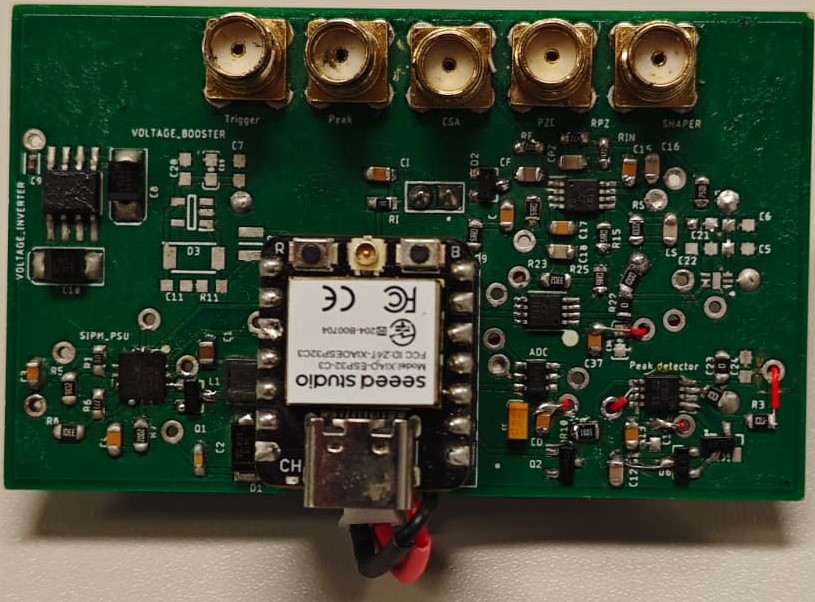
\includegraphics[width=186pt,height=127pt]{images/pcb_teste.jpg}};

% ---- Region outlines ---------------------------------------------------
\draw [reg,color={rgb, 255:red, 241; green, 74; blue, 64 }]
      (2.55,24.84) rectangle (52.93,59.98);                 % SiPM power supply
\draw [reg,color={rgb, 255:red, 26; green, 111; blue, 223 }]
      (116.09,72.67) rectangle (166.47,101.07);             % pulse shaping
\draw [reg,color={rgb, 255:red, 204; green, 153; blue, 0 }]
      (113.63,34.27) rectangle (129.67,53.47);              % ADC
\draw [reg,color={rgb, 255:red, 55; green, 173; blue, 107 }]
      (113.51,63.72) .. controls (118.22,73.60) and (139.09,68.88) .. (153.45,57.88)
   .. controls (167.81,46.87) and (177.68,49.12) .. (178.35,43.95)
   .. controls (179.03,38.79) and (182.39,38.56) .. (172.97,30.48)
   .. controls (163.55,22.40) and (163.98,22.18) .. (151.65,21.95)
   .. controls (139.33,21.72) and (126.97,19.26) .. (126.86,25.54)
   .. controls (126.74,31.83) and (140.14,43.95) .. (136.62,50.01)
   .. controls (133.10,56.08) and (108.80,53.84) .. (113.51,63.72) -- cycle ;

% ---- Labels over the board (no arrows) --------------------------------
\node [lbl,draw=none,font=\scriptsize,anchor=center] at (83.33,54.66) {MCU};
\node [lbl,draw={rgb, 255:red, 204; green, 153; blue, 0 },
       font=\scriptsize,anchor=center] at (114.30,27.04) {ADC};
\node [lbl,draw={rgb, 255:red, 241; green, 74; blue, 64 },anchor=center]
      at (27.90,13.25) {SiPM\\Power Supply};
\node [lbl,draw={rgb, 255:red, 55; green, 173; blue, 107 },anchor=center]
      at (163,13.25) {Pulse\\Discrimination};

% ---- Pulse shaping (right of the board) -------------------------------
\node [lbl,draw={rgb, 255:red, 26; green, 111; blue, 223 },anchor=west]
      at (165,86.90) {Pulse\\Shaping};



% ---- Signal test points (only arrow in the figure) --------------------
\node [lbl,draw={rgb, 255:red, 81; green, 81; blue, 81 },anchor=center]
      at (27.60,88) {Signal\\Test Points};
\draw [color={rgb, 255:red, 81; green, 81; blue, 81 },line width=1.1pt] (50,99) -- (50,108);
\draw [shift={(50,116)},rotate=270,ah,fill={rgb, 255:red, 81; green, 81; blue, 81 }]
      (7.85,-3.78) -- (0,0) -- (7.85,3.78) -- cycle ;

% ---- Width dimension (7 cm) --------------------------------------------
\draw [line width=1.1pt,black] (3.56,134) -- (184.42,134);
\draw [shift={(3.56,134)},rotate=0,ah,fill=black]
      (7.85,-3.78) -- (0,0) -- (7.85,3.78) -- cycle ;
\draw [shift={(184.42,134)},rotate=180,ah,fill=black]
      (7.85,-3.78) -- (0,0) -- (7.85,3.78) -- cycle ;
\node [dim,anchor=center] at (94,134) {7~cm};

% ---- Height dimension (4.3 cm) -----------------------------------------
\draw [line width=1.1pt,black] (-8,23.50) -- (-8,125.65);
\draw [shift={(-8,23.50)},rotate=90,ah,fill=black]
      (7.85,-3.78) -- (0,0) -- (7.85,3.78) -- cycle ;
\draw [shift={(-8,125.65)},rotate=270,ah,fill=black]
      (7.85,-3.78) -- (0,0) -- (7.85,3.78) -- cycle ;
\node [dim,anchor=center,rotate=90] at (-8,74.60) {4.3~cm};

\end{tikzpicture}}}
  \end{minipage}%
  \hfill%
  \begin{minipage}[c]{0.48\linewidth}
    \centering
    \subfloat[]{\label{fig:dori_case}%
      \resizebox{\linewidth}{!}{\begin{tikzpicture}[x=1pt,y=1pt,
    every node/.style={font=\footnotesize},
    ah/.style={draw opacity=0,line width=0.08,fill opacity=1},
    lbl/.style={fill=white,fill opacity=0.88,text opacity=1,
                align=center,inner sep=2.5pt,line width=0.6pt},
    dim/.style={fill=white,align=center,inner sep=2pt,draw=none,font=\scriptsize}]

% ---- Photograph -------------------------------------------------------
\node [anchor=south west,inner sep=0] at (0,0)
  {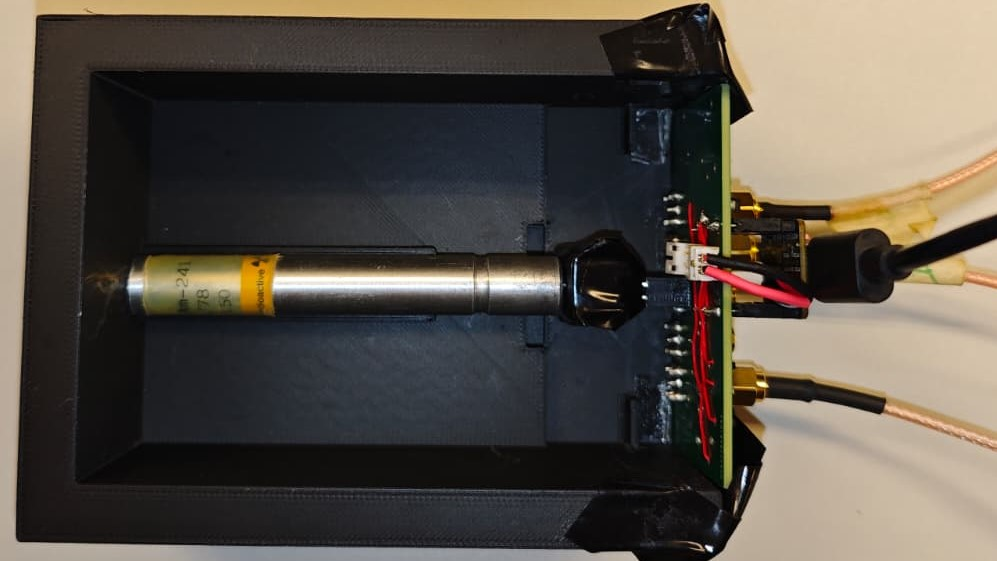
\includegraphics[width=200pt,height=127.1pt]{images/dori_case.jpg}};

% ---- 12 cm dimension (above the image, black) -------------------------
\draw [line width=1.1pt,black] (8.8,134) -- (144.4,134);
\draw [shift={(8.8,134)},rotate=0,ah,fill=black]
      (7.85,-3.78) -- (0,0) -- (7.85,3.78) -- cycle ;
\draw [shift={(144.4,134)},rotate=180,ah,fill=black]
      (7.85,-3.78) -- (0,0) -- (7.85,3.78) -- cycle ;
\node [dim,anchor=center] at (76.6,134) {12~cm};

% ---- Source holder -----------------------------------------------------
\node [anchor=south,align=center,
       text={rgb, 255:red, 204; green, 153; blue, 0 }] at (78,90) {Source Holder};
\draw [color={rgb, 255:red, 204; green, 153; blue, 0 },line width=1.1pt] (62,88) -- (58.15,79.2);
\draw [shift={(55,72)},rotate=66.4,ah,fill={rgb, 255:red, 204; green, 153; blue, 0 }]
      (7.85,-3.78) -- (0,0) -- (7.85,3.78) -- cycle ;
\draw [color={rgb, 255:red, 204; green, 153; blue, 0 },line width=1.1pt] (94,88) -- (100.4,80.5);
\draw [shift={(105.5,74.5)},rotate=130.4,ah,fill={rgb, 255:red, 204; green, 153; blue, 0 }]
      (7.85,-3.78) -- (0,0) -- (7.85,3.78) -- cycle ;

% ---- SiPM + scintillator ----------------------------------------------
\node [lbl,draw={rgb, 255:red, 26; green, 111; blue, 223 },anchor=north east]
      (sipm) at (196,112) {SiPM\\+\\Scintillator};
\draw [color={rgb, 255:red, 26; green, 111; blue, 223 },line width=1.1pt]
      (sipm.west) -| (118.1,77.4);
\draw [shift={(118.1,69.5)},rotate=90,ah,fill={rgb, 255:red, 26; green, 111; blue, 223 }]
      (7.85,-3.78) -- (0,0) -- (7.85,3.78) -- cycle ;

% ---- PCB ---------------------------------------------------------------
\node [lbl,draw={rgb, 255:red, 55; green, 173; blue, 107 },anchor=east]
      (pcb) at (196,49.9) {PCB};
\draw [color={rgb, 255:red, 55; green, 173; blue, 107 },line width=1.1pt]
      (pcb.west) -- (155.4,49.9);
\draw [shift={(147.5,49.9)},rotate=0,ah,fill={rgb, 255:red, 55; green, 173; blue, 107 }]
      (7.85,-3.78) -- (0,0) -- (7.85,3.78) -- cycle ;

% ---- 3D printed test box ----------------------------------------------
\node [lbl,draw={rgb, 255:red, 81; green, 81; blue, 81 },anchor=south east]
      (box) at (196,4) {3D Printed\\Test Box};
\draw [color={rgb, 255:red, 81; green, 81; blue, 81 },line width=1.1pt]
      (box.west) -- (131,15);
\draw [shift={(123,15)},rotate=0,ah,fill=black,
       fill={rgb, 255:red, 81; green, 81; blue, 81 }]
      (7.85,-3.78) -- (0,0) -- (7.85,3.78) -- cycle ;

\end{tikzpicture}}}
  \end{minipage}
  \caption[DORI-test board.]{%
    DORI-test board.
    \textbf{(a)} PCB with the main functional blocks identified, together with the signal test points used for characterisation;
    \textbf{(b)} assembled prototype inside the 3D printed test box, showing the sealed source holder aligned with the scintillator and SiPM.
  }
  \label{fig:pcb}
\end{figure}
\subsection{Pulse Shaping}
The current pulse produced by the SiPM delivers a quantity of charge, $Q$, that must be converted into a measurable voltage signal in the preamplifier~\cite{105}:
\begin{equation}
    Q = \int I(t)\, dt, \quad \text{unit: } [\mathrm{C}]
    \label{eq:charge}
\end{equation}

To achieve this, a Charge-Sensitive Amplifier (CSA) was implemented. The CSA is widely used as a preamplifier since the rise time of the output pulse depends only on the charge collection time in the detector, independent of both the detector and the preamplifier input capacitances~\cite{14}. It is an inverting integrator configuration designed around a low-noise operational amplifier, such as the LT6203~\cite{LT6202_LT6203_LT6204}, that was chosen accordingly. The feedback loop is closed by a capacitor $C_f$ in parallel with a resistor $R_f$~\cite{106,14}.

In this circuit, the current flows through $C_f$, allowing it to store charge and producing an output voltage proportional to $Q$. $R_f$ acts as a reset mechanism, providing a discharge path for $C_f$, in order for new pulses to be detected. The resulting output voltage can be written as~\cite{104,105}:
\begin{equation}
    V_{\text{out}} = -\frac{Q}{C_f}\, e^{-t/\tau_f}, \quad \text{unit: } [\mathrm{V}]
    \label{eq:vout}
\end{equation}

\noindent where $\tau_f = R_f C_f$ is the discharge time constant. For total
charge integration, this constant must be longer than the duration of the SiPM current pulse.

The charge gain of the CSA, $G$,  depends exclusively on $C_f$ and is therefore~\cite{106}:
\begin{equation}
    G = \frac{V_{\text{out}}}{Q} = -\frac{1}{C_f}, \quad \text{unit: } [\mathrm{V/C}]
    \label{eq:gain}
\end{equation}

To preserve the pulse amplitude, which carries the energy information of the detected events, additional signal conditioning stages were implemented. Given the high event count rate expected in IR, a Semi-Gaussian shaper was adopted in order to prevent baseline drift and relax the timing demands of the following stages. It consists of a CR differentiator followed by $n$ RC integrator stages. Increasing $n$ produces a more symmetric output pulse, which returns to baseline faster but introduces a longer peaking time~\cite{14}. For this work, a simple CR-RC ($n=1$) network was implemented, with equal differentiation and integration time constants.

The finite decay time constant of the CSA causes an undershoot at the shaper output~\cite{107}. If the signal has not recovered before the next event arrives, the subsequent pulse is superimposed on this undershoot, reducing its measured amplitude. To mitigate this effect, a Pole-Zero Cancellation (PZC) configuration was implemented. $C_{\text{diff}}$ and $R_{\text{diff}}$ form the CR differentiation network. A resistor $R_{\text{pz}}$, placed in parallel with $C_{\text{diff}}$, introduces a zero that compensates the pole produced by the CSA. Proper cancellation occurs when the following condition is satisfied~\cite{108,14,110}:
\begin{equation}
    R_{\text{pz}}\, C_{\text{diff}} = R_f\, C_f
    \label{eq:pzc}
\end{equation}

 The RC stage was implemented as an inverting low-pass filter, similar to the CSA configuration, with a feedback capacitor $C_s$ in parallel with a resistor $R_s$. As in the CSA, the gain depends on the feedback capacitor, so the value of $C_s$ controls the gain of the stage. The value of $R_s$ is then chosen so that $R_s C_s$ equals the common time constant fixed by the previous stages.

The gain of the front-end electronics was set empirically. As mentioned in Section~\ref{sec:sipm_power_supply}, the SiPM bias was fixed to keep the dark count rate at a low amplitude without masking the low-energy end of the spectrum. The gain must be high enough that real pulses are resolved above this level. It must also be low enough that the full energy range of interest, up to 100~keV, remains below saturation. The gain therefore places the spectrum in the lower portion of the available 3.3 V amplitude range.
Within this portion, enough channels must remain available to sample these energies. Following Knoll~\cite{14}, a spectral feature is adequately sampled when its full width at half maximum (FWHM) spans at least five channels. Of the reference sources available for this work, $^{241}$Am is the only one that produces a resolvable photopeak in BC-408, at
59.5~keV. The reported energy resolution of BC-408 at this energy is 30 to 50\%~\cite{119,126,127}. The narrowest case, 30\%, corresponds to a FWHM of 17.9~keV and sets the more demanding limit. Five channels across this FWHM give a channel width of 3.6~keV, and therefore a minimum of 28 channels up to 100~keV. This is a lower bound on the channel count, below which the photopeak is undersampled and energy information is lost. However, it is worth noting that such a small number of channels would be impractical for spectral characterisation, and therefore for energy calibration.

The $^{241}$Am source was nevertheless used to guide the gain. The pulses generated by the source were observed directly on the oscilloscope, and the gain was adjusted so that they did not saturate the OpAmps. It was set to remain within an amplitude range that the ADC samples with a reasonable number of channels, leaving room for the higher energies up to 100~keV. Ultimately, the gain was chosen to give finer binning while still satisfying the condition imposed by the most limiting factor, the resolution of BC-408. The resulting component values of the pulse shaping chain are listed in Table~\ref{tab:frontend}.

\vspace{1em}
\refstepcounter{table}
\label{tab:frontend}
\noindent\textbf{Table~\thetable.} Component values of the pulse shaping chain.
\addcontentsline{lot}{table}{\protect\numberline{\thetable}Component values of the pulse shaping chain.}
\vspace{0.1em}
\begin{table}[H]
  \centering
  \setlength{\tabcolsep}{12pt}
  \renewcommand{\arraystretch}{1.5}
  \begin{tabular}{c c c c c c}
    \toprule
    \multicolumn{2}{c}{\textbf{CSA}} &
    \multicolumn{2}{c}{\textbf{PZC}} &
    \multicolumn{2}{c}{\textbf{Shaper}} \\
    \cmidrule(lr){1-2}\cmidrule(lr){3-4}\cmidrule(lr){5-6}
    \textbf{Parameter} & \textbf{Value} &
    \textbf{Parameter} & \textbf{Value} &
    \textbf{Parameter} & \textbf{Value} \\
    \midrule
    \multirow{3}{*}{\shortstack{$R_f$ \\[2.2em] $C_f$}} &
    \multirow{3}{*}{\shortstack{4.7 k$\Omega$ \\[2.2em] 100 pF}} &
    $R_{\text{diff}}$ & 4.7 k$\Omega$ &
    \multirow{3}{*}{\shortstack{$R_s$ \\[2.2em] $C_s$}} &
    \multirow{3}{*}{\shortstack{10 k$\Omega$ \\[2.2em] 47 pF}} \\
    & & $R_{\text{pz}}$ & 4.7 k$\Omega$ & & \\
    & & $C_{\text{pz}}$ & 100 pF & & \\
    \midrule
    $\tau$ & 470 ns & & 470 ns & & 470 ns \\
    \bottomrule
  \end{tabular}
\end{table}

\subsubsection{Transient Response}

The transient response of the shaping chain to a single $^{241}$Am event is shown in Fig.~\ref{fig:shaping_chain}. The associated time metrics, extracted over the full set of acquired waveforms, are summarised in Table~\ref{tab:shaping}.

The integration at the CSA produces a negative pulse, since the charge is collected onto $C_f$ in an inverting configuration, and this polarity is preserved through the differentiating network. The inverting topology adopted for the last integrating stage restores a positive output at the shaper, as required by the single-positive-supply operation of the subsequent stages. A residual undershoot is nevertheless observed at every stage, originating from the CSA. Its relative magnitude is not increased along the chain, which would be the case in the absence of $R_{pz}$. The gain at the final stage was decreased, so that events of this energy are sampled towards the lower end of the available bins, as discussed. The main effect of the shaping is the redistribution of the signal in time. The semi-Gaussian output is broader and the time taken to reach the maximum is increased from $147 \pm 28$~ns at the CSA output to $387 \pm 50$~ns at the shaper, even though the latter has a lower amplitude. The interval over which the signal remains within 90\% of its maximum is doubled, from $208 \pm 167$~ns to $400 \pm 154$~ns. These effects are intended, since the amplitude is retained through comparator logic, and a maximum that is both delayed and sustained reduces the timing demands imposed on both the hardware and firmware. Within a broad range of amplitudes, the total shaping time is consistent across events, as it is set by the time constants selected for this network. At the shaper output it is $1.96 \pm 0.09$~$\mu$s, and this is the pulse the subsequent stages discriminate and sample.

\begin{figure}[H]
  \centering
  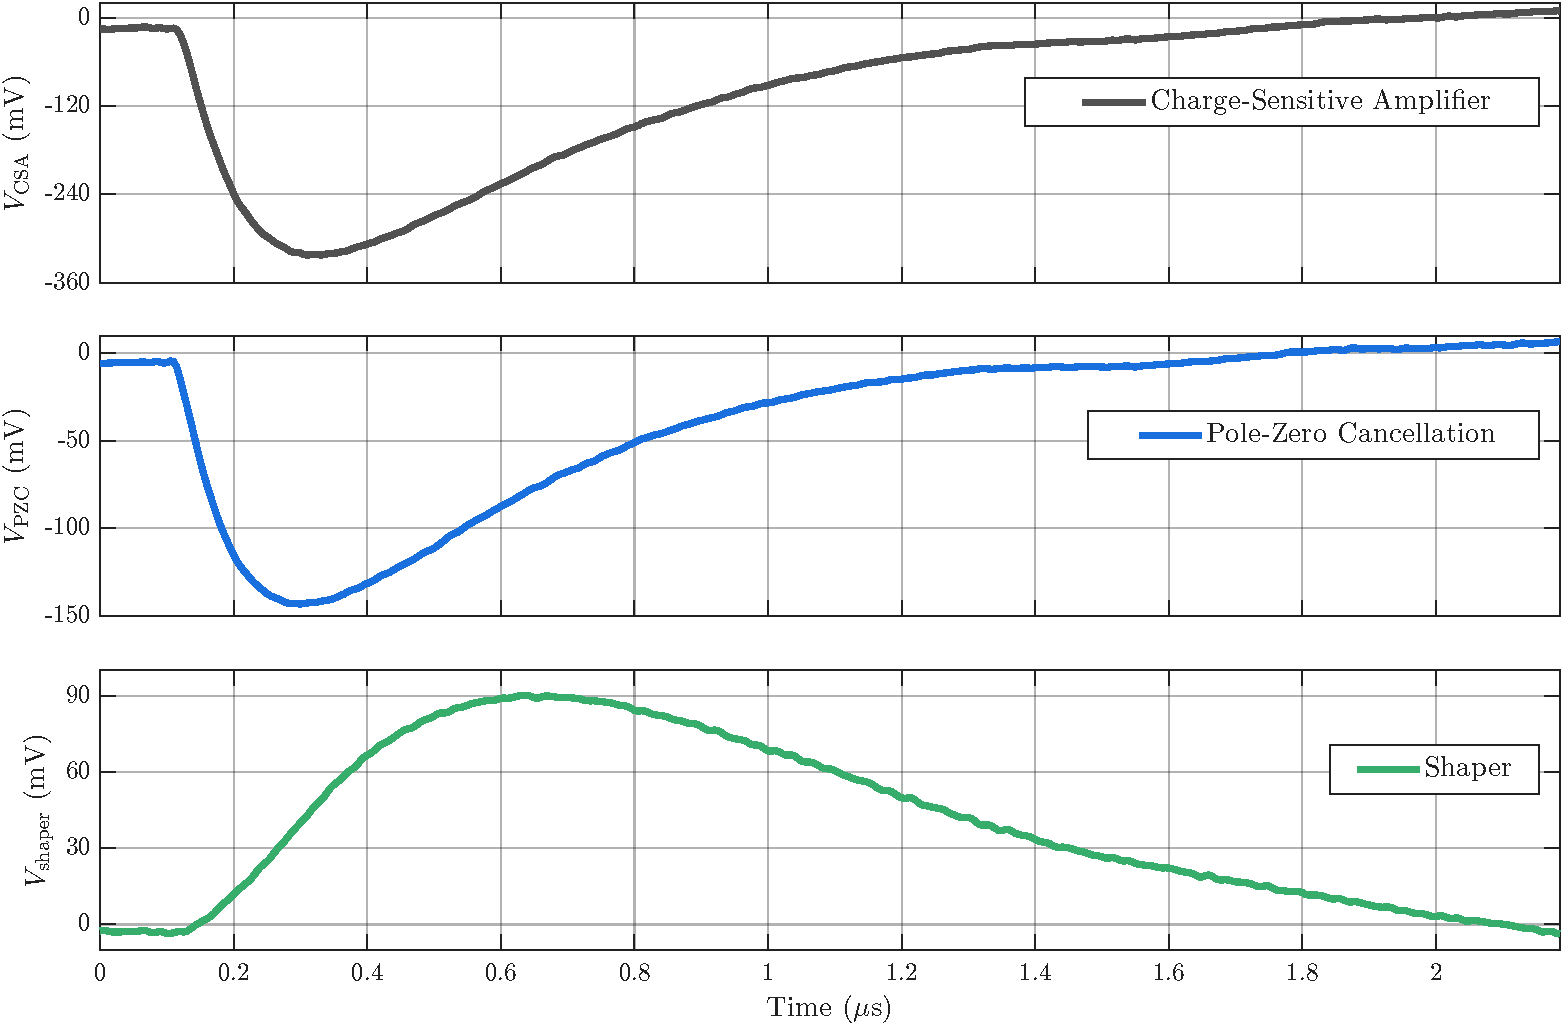
\includegraphics[width=\linewidth]{images/shaping_chain_trace00001.pdf}
  \caption[Transient response of the pulse shaping chain.]{Transient response of the CSA (grey), PZC (blue) and shaper (green) to a single $^{241}$Am event.}
  \label{fig:shaping_chain}
\end{figure}

\vspace{1em}

\refstepcounter{table}
\label{tab:shaping}
\noindent\textbf{Table~\thetable.} Timing metrics of the pulse shaping chain at each stage.
\addcontentsline{lot}{table}{\protect\numberline{\thetable}Timing metrics of the pulse shaping chain at each stage.}

\vspace{0.1em}

\begin{table}[H]
  \centering
  \setlength{\tabcolsep}{16pt}
  \renewcommand{\arraystretch}{1.65}
  \begin{tabular}{l c c c}
    \toprule
     & \textbf{CSA} & \textbf{PZC} & \textbf{Shaper} \\
    \midrule
    Amplitude range (mV)            & 191--861        & 87--430         & 61--407         \\
    Peaking time (ns)               & $147 \pm 28$    & $135 \pm 25$    & $387 \pm 50$    \\
    Width at 90\% of peak (ns)      & $208 \pm 167$   & $192 \pm 141$   & $400 \pm 154$   \\
    Total shaping time ($\mu$s)     & $1.42 \pm 0.09$ & $1.26 \pm 0.07$ & $1.96 \pm 0.09$ \\
    \bottomrule
  \end{tabular}
\end{table}


\subsection{Pulse Discrimination}
\label{sec:pulse_discrimination}

Pulse discrimination distinguishes real X-ray events from electronic noise and retains the amplitude of those accepted for digitisation. As mentioned above, it operates on a comparator logic. The LT1711~\cite{LT1711_LT1712} was selected for this application, a fast comparator operated in a non-inverting configuration. As shown in Fig.~\ref{fig:architecture}, the signal from the shaper is applied to the non-inverting input, while a fixed reference voltage, $V_{ref}$, is applied to the inverting input. The reference is derived from the 3.3 V supply rail through a resistive divider:

\begin{equation}
V_{ref} = \frac{R_2}{R_1 + R_2} \cdot 3.3, \text{ unit: [V]}
\label{eq:vref}
\end{equation}

\noindent where $R_1$ is the resistor connecting the node to the supply, and $R_2$ the resistor between the divider node and ground. The threshold was set to 10 mV. This value was established from the comparator input acquired under dark count conditions of the SiPM. The amplitudes of these events lie predominantly below 10 mV. The condition is satisfied by $R_1 = 33$ k$\Omega$ and $R_2 = 100$ $\Omega$.

A dedicated pin of the ESP32-C3 is connected to the logic output of the comparator and configured as an interrupt. Whenever the input exceeds $V_{ref}$, the comparator output switches to the logic high level. The pin is monitored continuously by dedicated hardware within the MCU, so the transition is registered as soon as it occurs. Detection initiates the readout loop, and the interrupt is detached for its duration, so that no further triggers are accepted while the event is being processed. It is reattached once the loop has terminated.

Simultaneously, the shaper output is fed to a Peak-and-Hold (P\&H) circuit. A P\&H captures the maximum of the input signal and sustains it after the pulse has decayed, extending the interval over which the peak amplitude remains available. The analogue conversion can then be performed more accurately. Given the small amplitude of the events, a configuration based on a precision rectifier is required. The adopted circuit is shown in Fig.~\ref{fig:peak_and_hold}. Two feedback paths are available to OA1. The outer path includes $D_2$ and runs from $C_H$ through the buffer OA2 and the resistor $R$ to the inverting input. The local path runs directly from the output of OA1 through $D_1$ to the same node. The two diodes are oppositely oriented, so only one path is closed at any instant, and the transition between them is determined by the position of the output of OA1 relative to the inverting input~\cite{Franco2015}.

With $C_H$ discharged and the shaped pulse rising, OA1 drives its output upwards. The anode of $D_2$ rises above its cathode, which is held at the capacitor voltage, so the diode becomes forward biased and conducts. Charge flows into $C_H$ and the capacitor voltage rises with the input. That voltage is read by OA2, and is returned through $R$ to the inverting input of OA1. Both amplifiers are implemented with the OPA354~\cite{OPA354}, whose input draws negligible current, so the stored charge cannot be drained by OA2. The amplifier therefore compares the shaped pulse against the stored voltage and continues to drive its output until the two coincide. $D_1$ is consequently reverse biased and its path is closed. This is the track mode, which is maintained until the pulse begins to decay~\cite{Franco2015}.

Once the maximum has passed, OA1 drives its output downwards. $D_2$ becomes reverse biased and the track loop is broken. At the same instant, the output of OA1 falls below the inverting input, $D_1$ becomes forward biased and establishes the local feedback path. Without this branch the amplifier would be left without feedback and driven into saturation against the negative supply, and recovery at the arrival of the following event would be governed by the slew rate. With $D_2$ reverse biased, the stored charge has no drain path through it. The remaining connections to the node are the input of OA2 and the reset path, which is held open throughout the interval. The peak value is therefore retained. This is the hold mode. The value of $C_H = 470$~pF, reflects a compromise between the two modes. A larger capacitance reduces droop during hold, but would take longer for OA1 to charge it, and higher pulses would not be held~\cite{Franco2015,Horowitz2015}.
\begin{figure}[H]
  \centering
  \tikzset{every picture/.style={line width=0.75pt}}

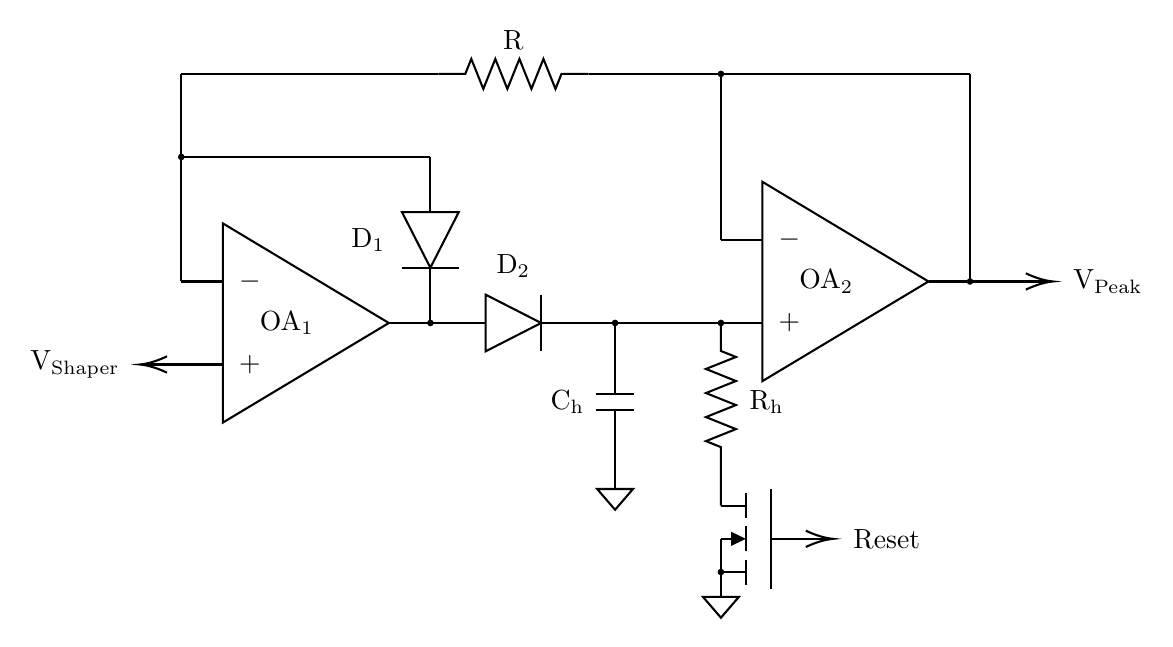
\begin{tikzpicture}[
    x=1.5pt, y=1.5pt, yscale=-1, xscale=1,
    every node/.style={font=\normalsize, inner sep=1pt}
]

%==================== Feedback resistor R (top rail) ====================
\draw    (200,40) -- (261.9,40) ;
\draw    (261.9,40) -- (268.41,40) -- (269.86,36.39) -- (272.76,43.61) -- (275.65,36.39) -- (278.55,43.61) -- (281.45,36.39) -- (284.35,43.61) -- (287.24,36.39) -- (290.14,43.61) -- (291.59,40) -- (298.1,40) ;
\draw    (298.1,40) -- (390,40) ;

%==================== OA_1 ====================
\draw    (210,76) -- (250,100) -- (210,124) -- cycle ;
\draw    (200,90) -- (210,90) ;
\draw    (210,110) -- (192,110) ;
\draw [shift={(190,110)}, rotate=0] [line width=0.75]
       (6.56,-1.97) .. controls (4.17,-0.84) and (1.99,-0.18) .. (0,0) .. controls (1.99,0.18) and (4.17,0.84) .. (6.56,1.97) ;
\draw    (200,40) -- (200,90) ;

%==================== D_1 (feedback diode) ====================
\draw    (200,60) -- (260,60) ;
\draw    (260,60) -- (260,73.31) ;
\draw    (266.83,73.31) -- (260,86.69) -- (253.17,73.31) -- cycle ;
\draw    (253.17,86.69) -- (266.83,86.69) ;
\draw    (260,86.69) -- (260,100) ;

%==================== D_2 (output diode) ====================
\draw    (250,100) -- (273.31,100) ;
\draw    (273.31,93.17) -- (286.69,100) -- (273.31,106.83) -- cycle ;
\draw    (286.69,93.17) -- (286.69,106.83) ;
\draw    (286.69,100) -- (340,100) ;

%==================== Hold capacitor C_h ====================
\draw    (304.5,100) -- (304.5,117) ;
\draw    (300,117) -- (309,117) ;
\draw    (300,121) -- (309,121) ;
\draw    (304.5,121) -- (304.5,140) ;
\draw    (300.19,140) -- (304.5,145) -- (308.81,140) -- cycle ;

%==================== Discharge resistor R_h ====================
\draw    (330,100) -- (330,106.74) -- (333.61,108.19) -- (326.39,111.08) -- (333.61,113.98) -- (326.39,116.88) -- (333.61,119.77) -- (326.39,122.67) -- (333.61,125.57) -- (326.39,128.46) -- (330,129.91) -- (330,144) ;

%==================== Reset MOSFET ====================
\draw    (336,141) -- (336,147) ;
\draw    (336,149) -- (336,155) ;
\draw    (336,157) -- (336,163) ;
\draw    (342,140) -- (342,164) ;
\draw    (342,152) -- (355,152) ;
\draw [shift={(357,152)}, rotate=180] [line width=0.75]
       (6.56,-1.97) .. controls (4.17,-0.84) and (1.99,-0.18) .. (0,0) .. controls (1.99,0.18) and (4.17,0.84) .. (6.56,1.97) ;
\draw    (330,144) -- (336,144) ;
\draw    (336,160) -- (330,160) ;
\draw    (330,152) -- (330,166) ;
\draw    (330,152) -- (334,152) ;
\draw [shift={(336,152)}, rotate=180] [fill={rgb, 255:red, 0; green, 0; blue, 0}, fill opacity=1] [line width=0.08] [draw opacity=0]
       (3.57,-1.72) -- (0,0) -- (3.57,1.72) -- cycle ;
\draw    (325.69,166) -- (330,171) -- (334.31,166) -- cycle ;

%==================== OA_2 ====================
\draw    (340,66) -- (380,90) -- (340,114) -- cycle ;
\draw    (330,40) -- (330,80) ;
\draw    (330,80) -- (340,80) ;
\draw    (380,90) -- (408,90) ;
\draw [shift={(410,90)}, rotate=180] [line width=0.75]
       (6.56,-1.97) .. controls (4.17,-0.84) and (1.99,-0.18) .. (0,0) .. controls (1.99,0.18) and (4.17,0.84) .. (6.56,1.97) ;
\draw    (390,40) -- (390,90) ;

%==================== Junction dots ====================
\fill (200,60)    circle (0.8) ;
\fill (260,100)   circle (0.8) ;
\fill (304.5,100) circle (0.8) ;
\fill (330,100)   circle (0.8) ;
\fill (330,40)    circle (0.8) ;
\fill (330,160)   circle (0.8) ;
\fill (390,90)    circle (0.8) ;

%==================== Labels ====================
% terminals
\draw (186,110) node [anchor=east] {V$_{\mathrm{Shaper}}$};
\draw (414,90)  node [anchor=west] {V$_{\mathrm{Peak}}$};
\draw (361,152) node [anchor=west] {Reset};

% op-amps
\draw (218,100) node [anchor=west] {OA$_{1}$};
\draw (213,90)  node [anchor=west] {$-$};
\draw (213,110) node [anchor=west] {$+$};
\draw (348,90)  node [anchor=west] {OA$_{2}$};
\draw (343,80)  node [anchor=west] {$-$};
\draw (343,100) node [anchor=west] {$+$};

% passives
\draw (280,35)  node [anchor=south] {R};
\draw (250,80)  node [anchor=east]  {D$_{1}$};
\draw (280,90)  node [anchor=south] {D$_{2}$};
\draw (298,119) node [anchor=east]  {C$_{\mathrm{h}}$};
\draw (336,119) node [anchor=west]  {R$_{\mathrm{h}}$};

\end{tikzpicture}
  \caption[Peak-and-Hold circuit.]{Peak-and-Hold circuit based on a precision rectifier. The outer feedback path of OA1 is shown at the top through $R$, while the local path closes through $D_1$.} 
  \label{fig:peak_and_hold}
\end{figure}

With no reset path, the capacitor would only ever accumulate charge. Once a maximum has been stored, a subsequent event of lower amplitude cannot forward bias $D_2$. The output would therefore converge to the largest amplitude ever received rather than to the amplitude of each individual event. A discharge path is therefore required, and it must be opened and closed under control so that $C_H$ is emptied between events. This function is performed by an N-channel MOSFET placed in series with $R_{H}=7.5$~k$\Omega$ across the capacitor, driven by a logic level from the MCU. When held low, the path between drain and source is open and the stored charge is retained. At the 3.3 V level the channel is established and the capacitor discharges through $R_H$ with a time constant $\tau = R_H C_H$. The gate is therefore held low by default, so that the circuit is always ready to capture the maximum of the signal. Detection of a valid pulse raises the interrupt described above, after which a delay of 2~$\mu$s is imposed to allow the held value to stabilise before the sampling logic is applied. The gate is then driven high for an interval longer than $\tau$, sufficient for $C_H$ to discharge, and returned low~\cite{Franco2015}.

\subsubsection{Transient Response}

The output of the pulse discrimination chain to a single $^{241}$Am event is shown in Fig.~\ref{fig:pulse_discrimination}. The trigger level was taken as the intersection between the shaper output and the comparator transition. It is measured at 9.3~mV, in agreement with the nominal threshold of approximately 10~mV. Upon reaching the maximum, the P\&H circuit retains the amplitude of the event, although a droop of the held value is present throughout the hold interval. The decay is more pronounced over the first two microseconds after the peak, which justifies the pre-sampling delay mentioned above. The residual droop over the rest of the hold is attributed to leakage through the capacitor, the diode and/or the reset path~\cite{Franco2015,Horowitz2015}.

No sampling logic was implemented for these measurements. Nevertheless, a latency is present in the transition of the transistor logical state. The hold interval is therefore extended beyond the value imposed by the firmware, which contributes directly to the dead time of the detector. Once the reset path is closed, the discharge of the storage capacitor is governed by the time constant imposed by $R_h$ and $C_h$. It was observed, however, that the output does not return to ground, settling instead at a residual baseline of approximately 50~mV. The discharge also continues after the gate has returned to the low logical state, at which point the capacitor should retain its stored voltage. This is consistent with the transition latency described above. It was first considered whether $R_h$ was too high for the discharge to complete within the time the gate sits at 3.3~V. To assess this, $R_h$ was changed to 1~k$\Omega$. Although the discharge was completed in a shorter interval, as expected, the output would settles at the same residual baseline. This behaviour could be justified with the single-supply configuration of the OpAmps. With the negative rail of OA1 connected directly to ground, the amplifier cannot reproduce the negative baseline of the shaper output. Once the reset path is open, and the input at OA1 remains negative, the current needed to supply this load may cause an output swing. This output swing would be the floor at which $C_h$ can be minimally charged. Therefore, no event below 50~mV can be sampled, as it cannot be tracked. It is a limitation of the current front-end electronics, and it reduces the dynamic range available at the lower end of the energies of interest. Ultimately, $R_h$ was kept at 7.5~k$\Omega$. Without sampling logic, the mean dead time is measured as 13~$\pm$~1~$\mu$s, taken as the interval over which the P\&H output remains at hold until it discharges to the residual baseline.

\begin{figure}[H]
  \centering
  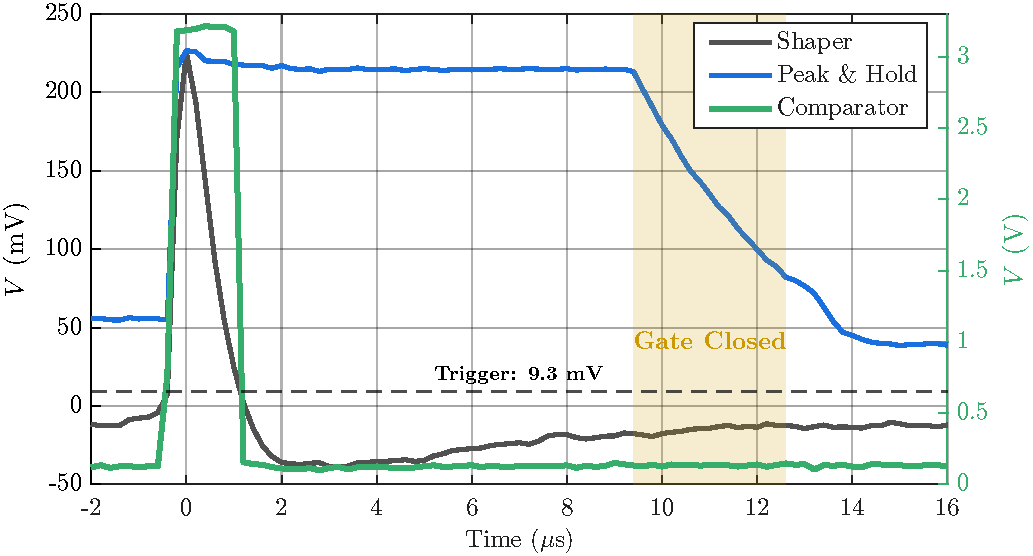
\includegraphics[width=\linewidth]{images/7.5k_notitle.pdf}
  \caption[Transient response of the pulse discrimination chain.]{Transient response of the shaper (grey), comparator (green) and P\&H (blue) stages to a single $^{241}$Am event. The yellow region marks the interval during which the reset transistor is driven HIGH, allowing the hold capacitor to discharge.}
  \label{fig:pulse_discrimination}
\end{figure}

\subsection{Pulse Sampling}
\label{sec:pulse_sampling}
Pulse sampling digitises the held signal through an ADC. The converter maps the input range onto $2^n$ discrete levels, where $n$ is its resolution in bits. Each amplitude is sampled and quantized to a corresponding digital bin. Since the conversion occupies the acquisition
chain, the introduction of a sampling stage is expected to increase the dead time of DORI. Two converters were therefore evaluated, the ADC internal to the ESP32-C3 and an external ADS7883~\cite{ADS7883}, both of 12-bit resolution. The measured dead times are presented in Table~\ref{tab:dead_time}.

\vspace{1em}
\refstepcounter{table}
\label{tab:dead_time}
\noindent \textbf{Table \thetable.} Dead time of the acquisition chain for each sampling
condition. Values are the mean of multiple $^{241}$Am events with the corresponding standard
deviation.
\vspace{0.1em}
\begin{center}
\setlength{\tabcolsep}{22pt}
\renewcommand{\arraystretch}{1.3}
\begin{tabular}{ccc}
\hline
\textbf{Sampling Condition} & \textbf{Dead Time ($\mu$s)} & \textbf{Sampling Protocol} \\
\hline
\textit{N/A} & 13.2 $\pm$ 0.9 & \textit{N/A} \\
Internal MCU ADC & 59.2 $\pm$ 1.5 & Analog Read \\
External ADC & 17.8 $\pm$ 0.4 & SPI \\
\hline
\end{tabular}
\end{center}
\vspace{1em}

From the perspective of power consumption and component complexity, the internal converter would be preferable. However, relative to the dead time measured without a sampling stage, the internal converter adds a delay ten times higher than the external one. The internal ADC is accessed through the \texttt{analogRead} routine, and limited by its own execution time, making it unsuitable for this application. On the other hand, the ADS7883 is read over SPI at 20~MHz, a dedicated high-speed protocol, and consequentely increasing the dead time by only 4.6~$\mu$s. The external converter was therefore adopted, as it allows a higher count rate to be achieved. The digitised values are subsequently rebinned to a 10-bit range in order to reduce the volume of data transmitted by the communication protocol. Over the 3.3~V input range, the resulting 1024 channels correspond to a channel width of 3.2~mV, which sets the smallest amplitude difference that can be resolved. With a dead time of 17.8~$\pm$~0.4~$\mu$s, the maximum count rate of DORI is $(56~\pm~1)\times10^{3}$~counts per second.


\section{Validation of the Front-End Electronics}
\label{sec:frontend-validation}
Prior to energy calibration of the PS, the readout electronics were validated using a $5 \times 5 \times 10$~mm CsI(Tl) crystal. The linearity of DORI can be tested by relating pulses of known energy to the channels in which they are stored. To identify an incident radionuclide emitting $\gamma$-rays, that is, to obtain the known energy pulse, photoelectric absorption must be favoured. An inorganic scintillator is appropriate for this validation owing to its higher density and effective atomic number, which favour photoelectric absorption in the energy range of interest. A linear channel-to-energy mapping is expected, and any significant deviation would be attributable to the front-end electronics~\cite{14}. This validation therefore indicates whether the front-end electronics introduce any non-linearity, such as the amplitude droop in the P\&H or its residual baseline. Should either prove amplitude-dependent, it would require characterisation or correction.

The hardware gain was adjusted to accommodate the higher light output of CsI(Tl), and spectra were acquired over 10-minute intervals using the three radioactive sources described previously. The resulting pulse height spectra are shown in Fig.~\ref{fig:validation_electronics} (a). The background was subtracted, and channels 18 and below were excluded, as its elevated count rate would otherwise dominate the vertical scale. Given the ADC step, channel 18 corresponds to a voltage of approximately 58~mV, which lies near the residual baseline of the P\&H stage. It can therefore be concluded that any event below this level is assigned to this bin, owing to the return of the hold capacitor to that charge. This does not compromise the validation, since all expected spectral features are resolved for each source, including the low energy 14.4~keV $\gamma$-ray emission of $^{57}$Co. The consequence is the masking of lower energies, and the implication for the PS calibration is that the energy range proposed must lie above this threshold.
\begin{figure}[H]
  \centering
  \subfloat[]{\label{fig:spectra}%
    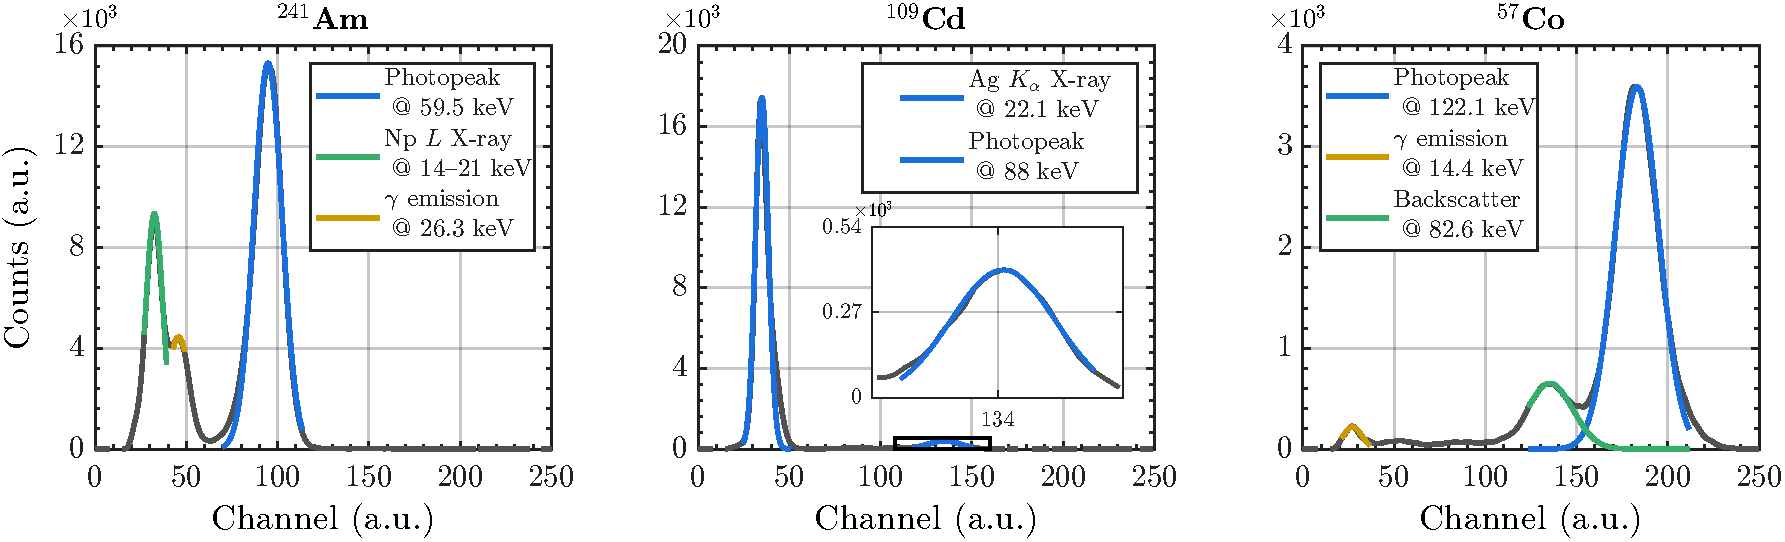
\includegraphics[width=\linewidth]{images/spectra.pdf}}\\[1ex]
  \subfloat[]{\label{fig:calib}%
    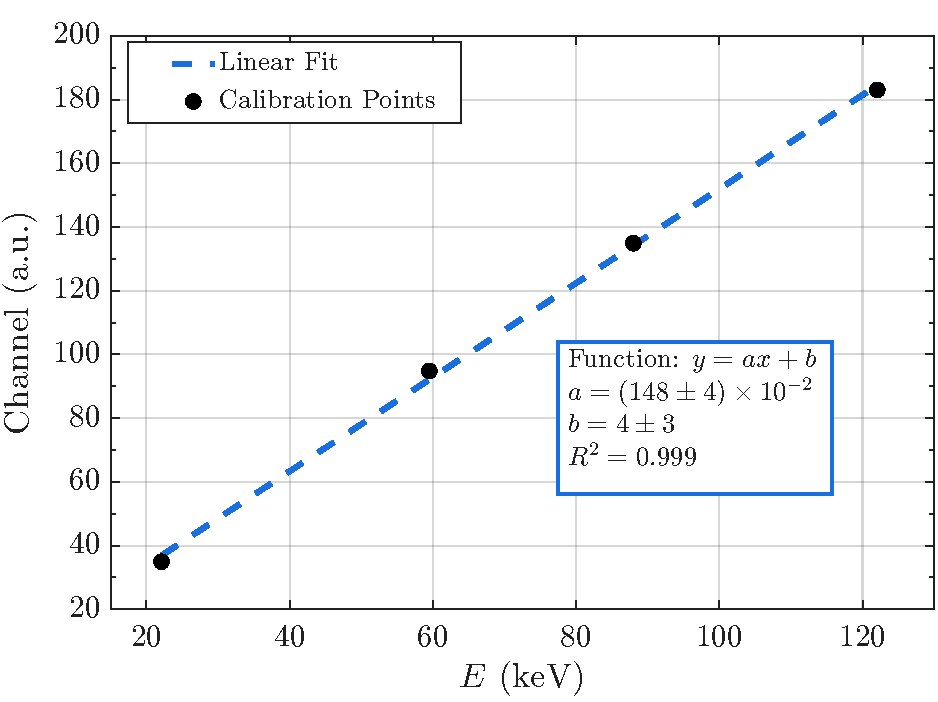
\includegraphics[width=0.47\linewidth]{images/fit_csi.pdf}}%
  \hfill%
  \subfloat[]{\label{fig:co57}%
    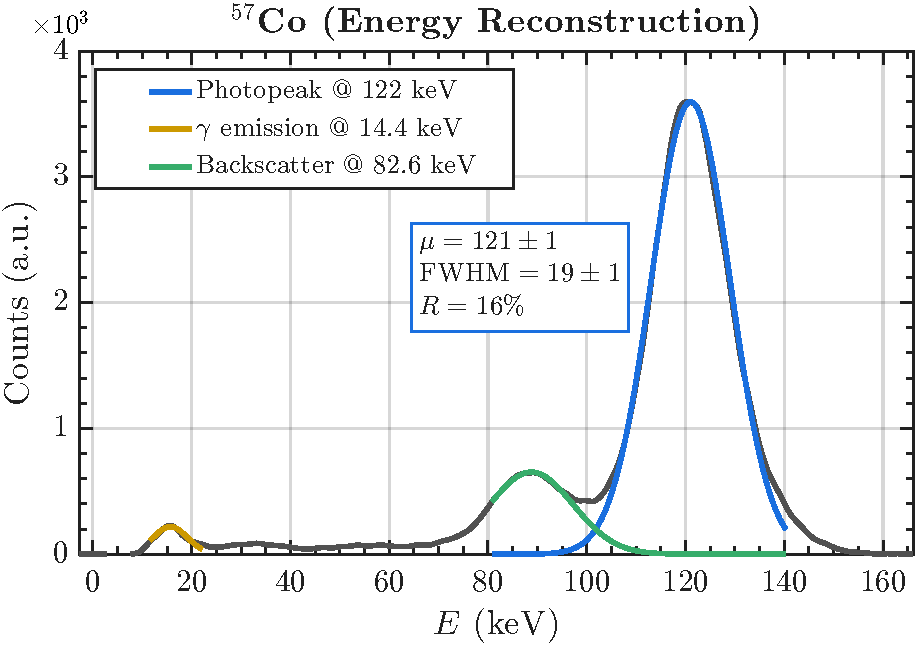
\includegraphics[width=0.50\linewidth]{images/co57_energy_reconstruction.pdf}}
  \caption[Validation of the Front-End Electronics.]{%
    \textbf{(a)} Pulse height spectra acquired with the CsI(Tl) crystal for the three calibration sources. Identified spectral features are labelled.
    \textbf{(b)} Channel-to-energy calibration curve with linear fit.
    \textbf{(c)} $^{57}$Co spectrum reconstructed in energy units.}
  \label{fig:validation_electronics}
\end{figure}

The centroid channel of each photopeak was mapped to its known energy value, and a linear fit of the form:
%
\begin{equation}
    C = aE + b,
    \label{eq:calibration_csi}
\end{equation}
%
was applied, where $C$ is the channel number and $E$ is the energy in keV (Fig.~\ref{fig:validation_electronics} (b)). The fit yields $R^2 = 0.999$, confirming a linear channel-to-energy relationship up to at least channel 183, corresponding to an input amplitude of approximately 590~mV. This confirms that the P\&H circuit does not introduce amplitude-dependent errors within this bin range.

As a validation of the calibration, the $^{57}$Co spectrum was reconstructed in energy units and is shown in Fig.~\ref{fig:validation_electronics} (c). The fitted centroid of the 122~keV photopeak yields $\mu = 121 \pm 1$~keV, consistent with the nominal value within uncertainty. The measured FWHM is $19 \pm 1$~keV, corresponding to an energy resolution of $16 \pm 1$\% at 122~keV, consistent with values reported in the literature for CsI(Tl)~\cite{117,118}. This indicates that the front-end electronics do not degrade the intrinsic energy resolution of the crystal. The DORI hardware is therefore considered validated.


